\documentclass[11pt,a4paper]{article}

% ---------------------------------------------------------------------------
% ThreatInt — technical research report
% ---------------------------------------------------------------------------
\usepackage[T1]{fontenc}
\usepackage[utf8]{inputenc}
\usepackage{lmodern}
\usepackage[margin=2.2cm,top=2.6cm,bottom=2.4cm]{geometry}
\usepackage{graphicx}
\usepackage{booktabs}
\usepackage{array}
\usepackage{tabularx}
\usepackage{longtable}
\usepackage{colortbl}
\usepackage{xcolor}
\usepackage{titlesec}
\usepackage{fancyhdr}
\usepackage{enumitem}
\usepackage{amsmath}
\usepackage{amssymb}
\usepackage{caption}
\usepackage{tcolorbox}
\usepackage{listings}
\usepackage[hidelinks]{hyperref}
\tcbuselibrary{skins,breakable}

% -- palette ---------------------------------------------------------------
\definecolor{navy}{HTML}{1B3A5C}
\definecolor{steel}{HTML}{34668C}
\definecolor{sky}{HTML}{5B9BD5}
\definecolor{crimson}{HTML}{C0392B}
\definecolor{amber}{HTML}{E08A1E}
\definecolor{forest}{HTML}{2E8B57}
\definecolor{grey}{HTML}{8A99A8}
\definecolor{paper}{HTML}{F7F9FB}
\definecolor{ink}{HTML}{1D2733}

% -- styling ---------------------------------------------------------------
\titleformat{\section}{\normalfont\Large\bfseries\color{navy}}{\thesection}{0.7em}{}
\titleformat{\subsection}{\normalfont\large\bfseries\color{steel}}{\thesubsection}{0.6em}{}
\titleformat{\subsubsection}{\normalfont\normalsize\bfseries\color{ink}}{\thesubsubsection}{0.5em}{}
\titlespacing*{\section}{0pt}{1.4em}{0.6em}

\pagestyle{fancy}
\fancyhf{}
\renewcommand{\headrulewidth}{0.4pt}
\renewcommand{\footrulewidth}{0pt}
\fancyhead[L]{\footnotesize\color{grey}ThreatInt --- Technical Research Report}
\fancyhead[R]{\footnotesize\color{grey}\thepage}

\captionsetup{font=small,labelfont={bf,color=navy},justification=centering}

\newtcolorbox{keybox}[1][]{
  colback=paper, colframe=steel, boxrule=0.8pt, arc=2pt,
  left=8pt, right=8pt, top=6pt, bottom=6pt,
  breakable, fonttitle=\bfseries\color{white}, coltitle=white,
  colbacktitle=steel, title=#1
}

\newtcolorbox{notebox}[1][]{
  colback=amber!6, colframe=amber, boxrule=0.7pt, arc=2pt,
  left=8pt, right=8pt, top=6pt, bottom=6pt, breakable,
  fonttitle=\bfseries\color{white}, coltitle=white,
  colbacktitle=amber, title=#1
}

\lstset{
  basicstyle=\ttfamily\footnotesize,
  backgroundcolor=\color{paper},
  frame=single, rulecolor=\color{grey!50},
  keywordstyle=\color{steel}\bfseries,
  stringstyle=\color{forest},
  commentstyle=\color{grey}\itshape,
  numbers=left, numberstyle=\tiny\color{grey}, numbersep=8pt,
  breaklines=true, showstringspaces=false,
  columns=fullflexible, keepspaces=true,
  xleftmargin=14pt, framexleftmargin=12pt,
}

\newcommand{\code}[1]{\texttt{\small #1}}
\newcommand{\fmono}[1]{\texttt{#1}}

% ---------------------------------------------------------------------------
\begin{document}

% ============================== TITLE PAGE =================================
\begin{titlepage}
\pagecolor{navy}
\color{white}
\centering
\vspace*{3.2cm}

{\fontsize{15}{18}\selectfont\color{sky}\textsc{Technical Research Report}}\\[0.8cm]
{\fontsize{40}{46}\selectfont\bfseries ThreatInt}\\[0.5cm]
{\fontsize{17}{21}\selectfont\color{white!88} An Automated Threat-Intelligence Pipeline}\\[0.25cm]
{\fontsize{13.5}{17}\selectfont\color{white!75}
Collection · Cross-Verification · ML Classification · Campaign Clustering}\\[2.2cm]

\rule{11cm}{0.6pt}\\[0.8cm]

{\fontsize{12}{15}\selectfont\color{white!85}
\textbf{Repository:} \texttt{Ashwin-kumar-jonjale/ThreatInt}\\[0.3cm]
\textbf{Branch:} \texttt{feat/threat-intel-pipeline}\\[0.3cm]
\textbf{Artifact:} \texttt{threatint} v0.1.0 · MIT licence\\[0.3cm]
\textbf{Stack:} Python 3.10+ · scikit-learn · Flask · Docker · GitHub Actions}

\vfill

{\fontsize{10}{13}\selectfont\color{white!65}
Every quantitative figure in this report is derived from a real, deterministic
offline run of the pipeline (seed 42). No numbers are illustrative.\\[0.4cm]
Compiled with \LaTeX{} · \today}

\end{titlepage}
\pagecolor{white}
\color{ink}

% ============================== TOC ========================================
\pagenumbering{roman}
\tableofcontents
\newpage
\pagenumbering{arabic}

% ============================== 1. EXEC SUMMARY ============================
\section{Executive Summary}

Security operations centres are drowning in alerts. A single analyst may be
expected to cross-check hundreds of indicators-of-compromise (IOCs) per day
against a dozen overlapping feeds, reconcile their disagreements by hand, and
decide what is genuinely malicious. The work is repetitive, slow, and
error-prone: the same indicator appears in five feeds with five different
labels, and the analyst's real value --- judgement and context --- is spent on
mechanical reconciliation.

\textbf{ThreatInt} is a complete, reproducible pipeline that automates that
mechanical layer end to end. It collects indicators from multiple trusted
sources, normalises and deduplicates them, scores the \emph{reliability of each
source} against the cross-source consensus, classifies each indicator with a
supervised machine-learning model, and clusters the malicious ones into
\emph{attack campaigns} using unsupervised density-based clustering. The output
is an analyst-facing console report, machine-readable JSON/CSV, and an
interactive web dashboard.

\begin{keybox}[Headline results --- offline reference run]
\begin{tabularx}{\linewidth}{@{}lX@{}}
\textbf{106} raw records ingested from \textbf{5} feeds &
\textbf{81} unique indicators after dedup \\
\textbf{13} indicators corroborated by $\geq 2$ sources &
\textbf{57} classified malicious, \textbf{24} benign \\
\textbf{8} attack campaigns discovered &
classifier \textbf{acc 0.860 · F1 0.850 · AUC 0.946} \\
\end{tabularx}
\end{keybox}

\noindent The design makes three deliberate bets that distinguish it from a
naive feed aggregator:

\begin{enumerate}[leftmargin=1.4em,itemsep=2pt]
  \item \textbf{Trust is computed, not assumed.} Each feed's static analyst
        prior is blended with dynamic signals (precision, recall, pairwise
        agreement, volume) measured against the consensus. An indicator's
        score is then the reliability-weighted vote of the feeds reporting it,
        with a saturating bonus for independent corroboration.
  \item \textbf{The pipeline is reproducible and network-optional.} Every
        collector supports a bundled fixture path and degrades gracefully to it
        on any fetch failure. The whole system runs offline, deterministically,
        in CI --- which is what makes the evaluation in this report trustworthy.
  \item \textbf{The ML is interpretable.} Features are human-legible (entropy,
        suspicious-TLD flag, phishing-keyword count, port risk), so the model's
        decisions can be explained to an analyst rather than black-boxed.
\end{enumerate}

% ============================== 2. INTRODUCTION ============================
\section{Introduction and Problem Statement}

\subsection{The analyst bottleneck}
Threat intelligence arrives as a firehose of partially-overlapping feeds:
domain blocklists, URL blacklists, phishing registries, honeypot captures,
malware-family trackers. Three structural problems make manual triage
expensive:

\begin{description}[leftmargin=1.2em,itemsep=3pt]
  \item[Volume] Thousands of new IOCs per day across feeds, far exceeding
    human review capacity.
  \item[Disagreement] Feeds overlap inconsistently. The same domain may be
    flagged by one feed and ignored by four others, with no obvious way to
    weigh whose judgement matters.
  \item[Fragmentation] Related indicators arrive as scattered, unconnected
    rows. A single campaign --- say, a phishing kit using five lookalike
    domains and a shared C2 IP --- is invisible unless something groups it.
\end{description}

\subsection{What the system must do}
ThreatInt targets exactly these three problems with three corresponding
capabilities, wrapped in one deterministic pipeline:

\begin{center}
\begin{tabularx}{\linewidth}{@{}>{\raggedright\arraybackslash}p{4.3cm}X@{}}
\toprule
\rowcolor{paper}\textbf{Problem} & \textbf{Capability} \\
\midrule
Volume & Automated collection from multiple feeds, normalised and deduplicated \\
Disagreement & Cross-verification: per-source reliability + consensus scoring \\
Fragmentation & ML classification + DBSCAN campaign clustering \\
\bottomrule
\end{tabularx}
\end{center}

\subsection{Scope and non-goals}
ThreatInt is an \emph{aggregation, scoring and grouping} system. It deliberately
does not fetch live malware, perform active scanning, or make blocking
decisions. Its outputs are advisory: ranked indicators, confidence scores, and
campaign groupings for a human to act on. This keeps the blast radius small and
the system auditable.

% ============================== 3. DESIGN ==================================
\section{Design Goals and Principles}

The codebase is small (2{,}246 lines of Python across 18 modules) but the
design decisions behind it are load-bearing. Six principles shaped it:

\begin{enumerate}[leftmargin=1.4em,itemsep=3pt]
  \item \textbf{Plain data structures over frameworks.} The core entities are
    \code{dataclasses} (\code{RawRecord}, \code{Observation}, \code{Indicator},
    \code{Campaign}, \code{SourceReliability}), not ORM or framework objects.
    Stages communicate by passing lists of these; nothing shares mutable global
    state. This makes every stage independently testable and reorderable.
  \item \textbf{Network-optional by construction.} A collector's contract is
    ``return \code{RawRecord}s, never assume the network.'' Every source has a
    bundled fixture, and \code{HttpCollector} falls back to it on \emph{any}
    exception. Offline runs are the default for tests and the dashboard.
  \item \textbf{Determinism.} A single \code{random\_seed} (42) governs corpus
    generation, the train/test split, and the classifier. The same run yields
    the same numbers --- the precondition for the evaluation here.
  \item \textbf{Separation of collection from interpretation.} Collectors emit
    source-specific records; a dedicated normalisation layer canonicalises
    them. A new feed is added by writing one parser, not by touching the ML.
  \item \textbf{Interpretability first.} Features and source scores are chosen
    so a human can read them. The model is a random forest with Gini
    importances, not an opaque embedder.
  \item \textbf{Fail soft, never fail the run.} A single bad feed must not abort
    the pipeline. Collection is wrapped per-source; model persistence is
    best-effort; the API clamps its inputs.
\end{enumerate}

% ============================== 4. ARCHITECTURE ============================
\section{System Architecture}

ThreatInt is organised as four horizontal layers sitting on a shared data
model, with three entry points on top. The architecture figure below shows the
whole system at a glance.

\begin{figure}[htbp]
\centering
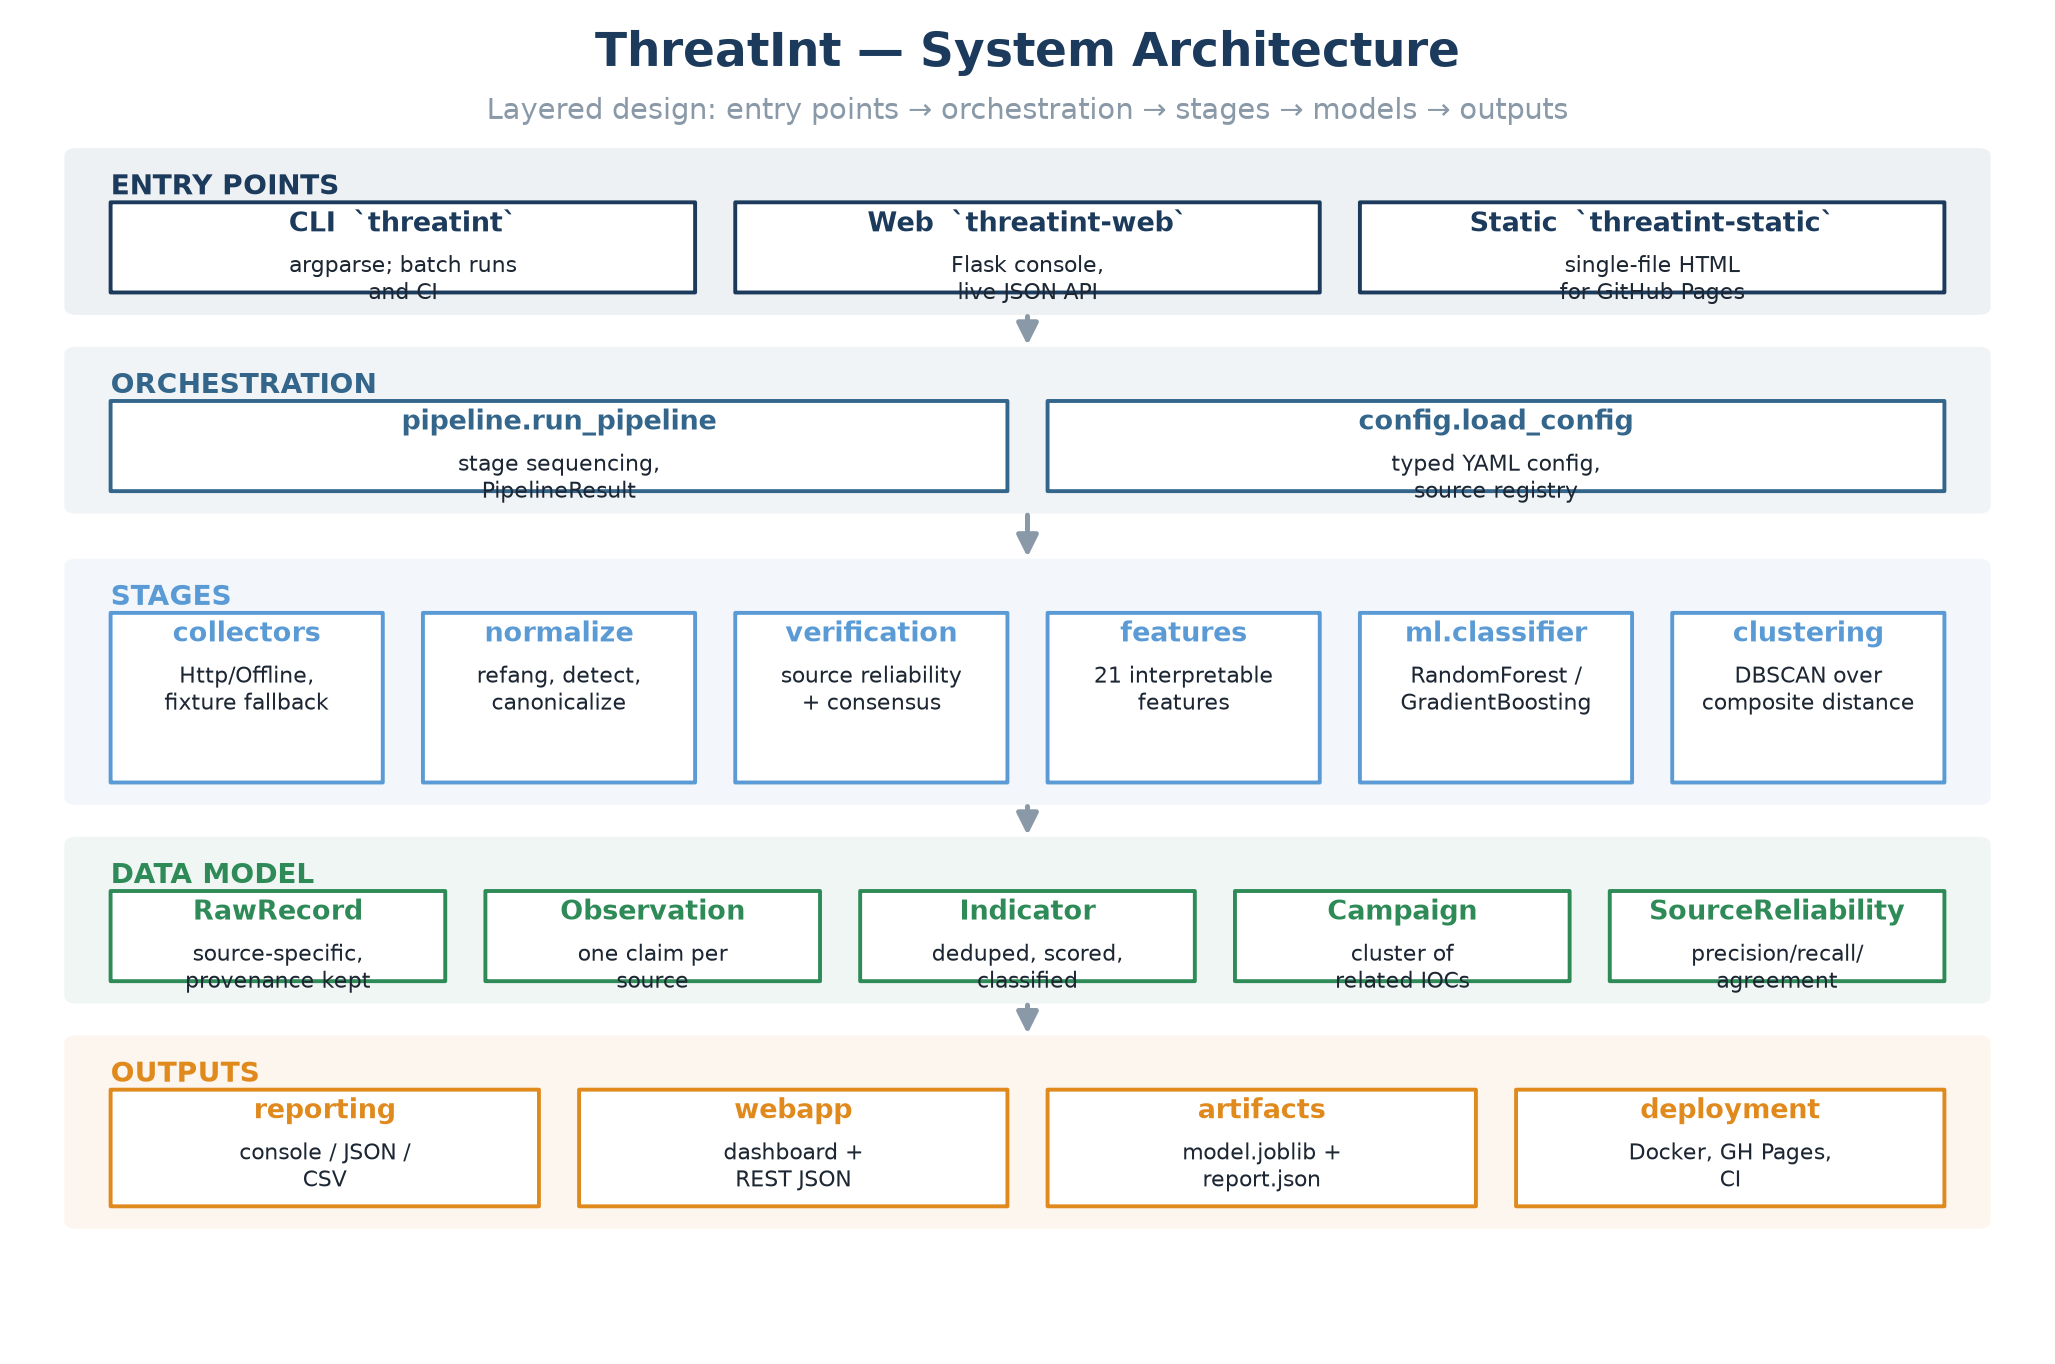
\includegraphics[width=\linewidth]{figures/fig1_architecture.png}
\caption{System architecture. Three entry points (CLI, live web console, static
export) drive a shared orchestrator, which sequences six pipeline stages over a
common data model and emits reports, a dashboard and persisted artifacts.}
\label{fig:arch}
\end{figure}

\subsection{The pipeline}
Orchestration lives in \code{pipeline.run\_pipeline}, which executes seven
ordered stages. Each stage is a small function owning no global state, so a run
is fully described by its \code{PipelineResult}. Figure~\ref{fig:flow} annotates
the stages with live counts from the reference run.

\begin{figure}[htbp]
\centering
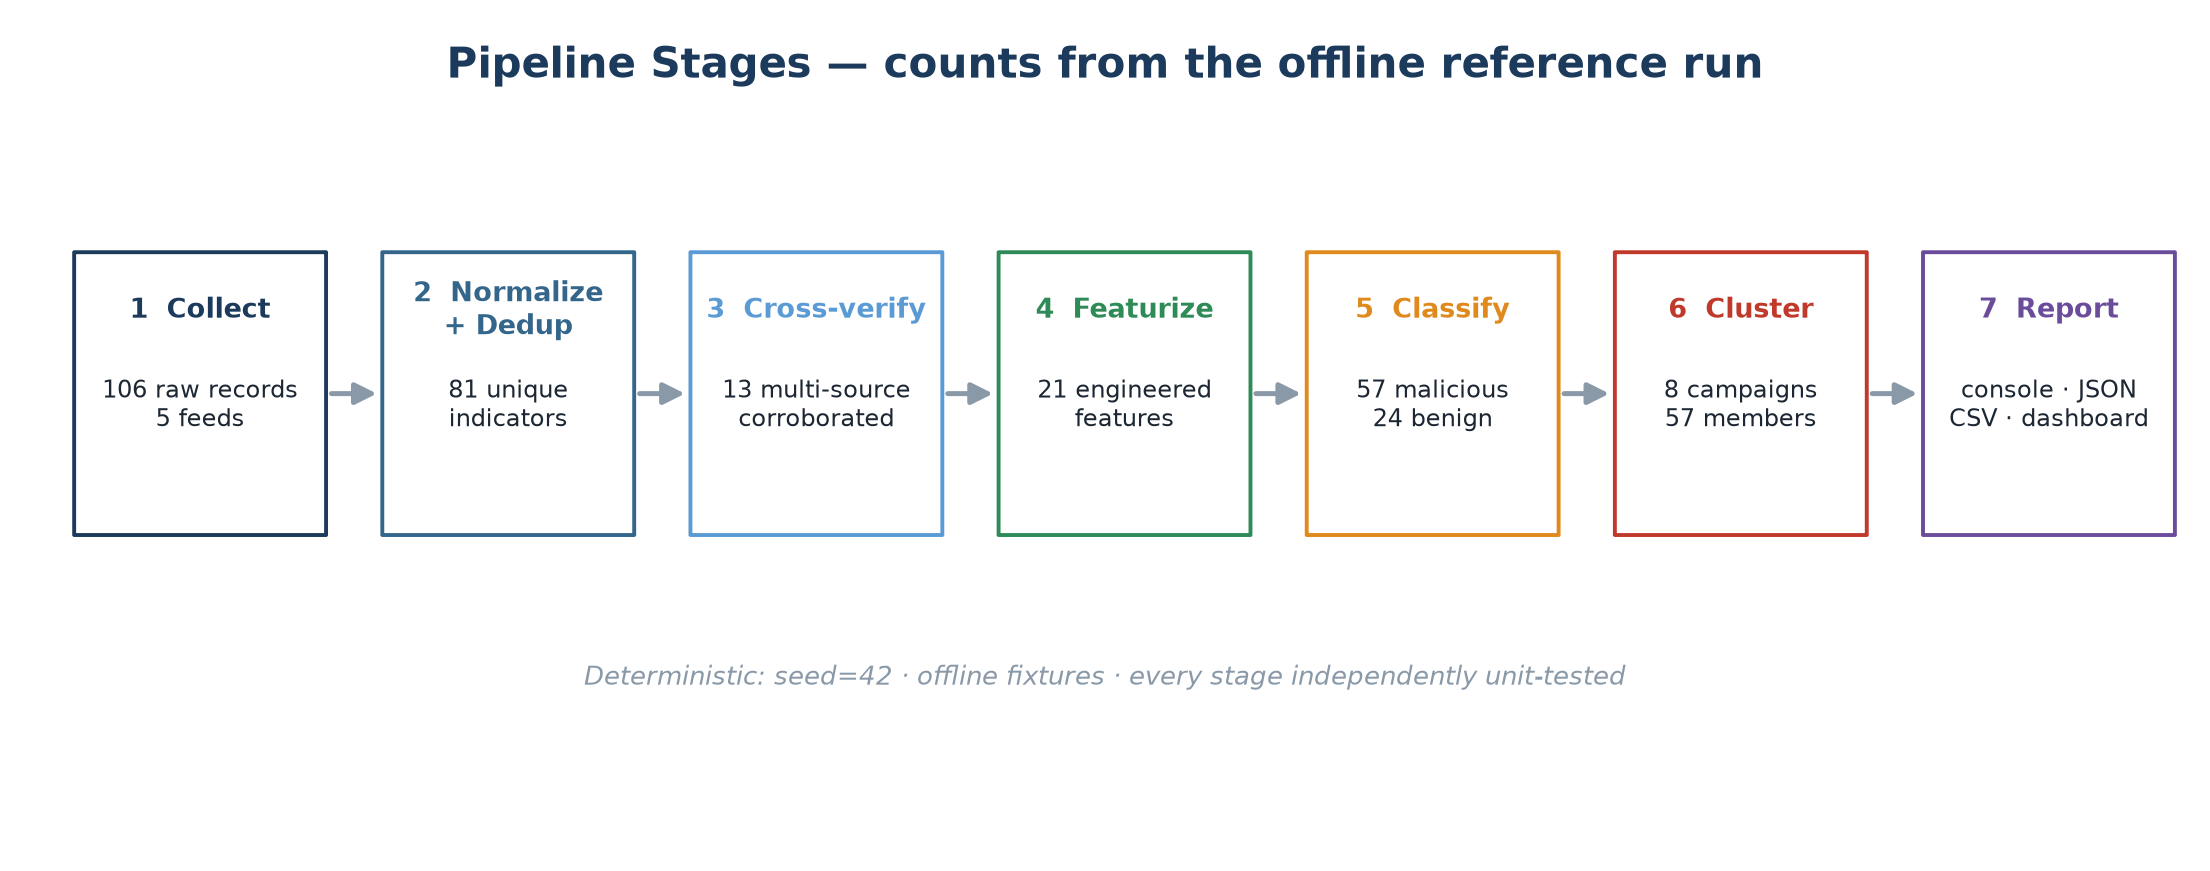
\includegraphics[width=\linewidth]{figures/fig2_pipeline_flow.png}
\caption{The seven pipeline stages with counts from the offline reference run.
Collect and verify collapse raw records into deduplicated, reliability-scored
indicators; featurize/classify attach verdicts; cluster groups the malicious
ones into campaigns.}
\label{fig:flow}
\end{figure}

The stage sequence is:

\begin{center}
\begin{tabularx}{\linewidth}{@{}>{\bfseries}p{2.4cm}p{2.9cm}X@{}}
\toprule
\rowcolor{paper}\textbf{Stage} & \textbf{Module} & \textbf{Responsibility} \\
\midrule
Collect & \code{collectors/} & Instantiate a collector per enabled source; emit \code{RawRecord}s; degrade to fixtures on failure. \\
Verify & \code{verification/} & Score each source's reliability; collapse observations into scored, deduplicated \code{Indicator}s. \\
Featurize & \code{features/} & Attach a fixed 21-dimensional numeric vector to every indicator. \\
Classify & \code{ml/} & Train (or load) the classifier; set \code{malicious\_probability} and \code{verdict}. \\
Cluster & \code{clustering/} & DBSCAN over a composite distance; produce \code{Campaign}s and stamp members. \\
Report & \code{reporting/} & Console, JSON and CSV renderings. \\
Present & \code{webapp/} & Flask dashboard and static HTML export. \\
\bottomrule
\end{tabularx}
\end{center}

% ============================== 5. DATA MODEL ==============================
\section{The Data Model}

Five dataclasses in \code{models.py} define every shape that moves through the
system. The pipeline is essentially a sequence of transforms between them:
\code{RawRecord} $\rightarrow$ \code{Observation} $\rightarrow$
\code{Indicator} $\rightarrow$ \code{Campaign}.

\begin{center}
\begin{tabularx}{\linewidth}{@{}>{\bfseries}p{3.2cm}p{2.5cm}X@{}}
\toprule
\rowcolor{paper}\textbf{Type} & \textbf{Stage} & \textbf{Key fields and meaning} \\
\midrule
\code{RawRecord} & collect & \code{source, indicator, indicator\_type, observed\_at, tags, confidence, raw}. The \code{raw} dict preserves the original payload for provenance and re-runs. \\
\code{Observation} & verify & One source's claim: \code{source, indicator, indicator\_type, observed\_at, confidence, tags}. Many observations collapse to one indicator. \\
\code{Indicator} & verify--cluster & Deduplicated observable. \code{indicator\_id} is a stable hash of \code{(type, value)}; carries \code{source\_count}, \code{reliability\_score}, \code{verdict}, \code{malicious\_probability}, \code{campaign\_id}, \code{features}. \\
\code{SourceReliability} & verify & \code{prior, precision, recall, agreement, volume, score}. \\
\code{Campaign} & cluster & \code{campaign\_id, label, indicators, shared\_tags}, with derived \code{size}, \code{mean\_reliability}, \code{mean\_malicious\_probability}. \\
\bottomrule
\end{tabularx}
\end{center}

\begin{keybox}[Why \code{indicator\_id} is a hash]
The identifier is \code{sha256("type:value")[:16]}. Because it is a pure
function of the canonical type and value, the \emph{same} observable reported by
five feeds collapses to a single object with no coordination between collectors.
It is also stable across runs, so campaign IDs --- themselves derived from
member IDs --- are reproducible.
\end{keybox}

Two enumerations anchor the vocabulary: \code{IndicatorType} (\code{ipv4},
\code{domain}, \code{url}, \code{md5}, \code{sha256}) and \code{Verdict}
(\code{malicious}, \code{benign}, \code{unknown}).

% ============================== 6. MODULES =================================
\section{Module-by-Module Reference}

This section walks the codebase in execution order. Each module's public
functions are tabulated with their purpose and behaviour.

\subsection{\code{normalize.py} --- canonicalisation and extraction}
Threat feeds are messy: defanged notation (\code{hxxp://}, \code{1[.]2[.]3[.]4}),
mixed types in one column, URLs carrying credentials, inconsistent casing. This
module turns any of that into validated, canonical indicators.

\begin{center}
\begin{tabularx}{\linewidth}{@{}>{\ttfamily\small}p{4.4cm}X@{}}
\toprule
\rowcolor{paper}\textbf{Function} & \textbf{Purpose} \\
\midrule
refang(value) & Reverse common defanging (\code{hxxp}$\rightarrow$\code{http}, \code{[.]}$\rightarrow$\code{.}) so indicators can be parsed. \\
defang(value) & Safe-to-share rendering; used by the dashboard so live IOCs are never shown clickable. \\
canonicalize(value, type) & Return the canonical form or \code{None}. Lower-cases domains/hashes, strips ports off IPs, rebuilds URLs from parsed components, drops fragments. \\
detect\_type(value) & Best-effort inference of an indicator's type via ordered regex checks (URL $\rightarrow$ IP $\rightarrow$ hash $\rightarrow$ domain). \\
extract\_indicators(text) & Pull every indicator out of a free-text blob; URLs are matched first and their spans excluded so a URL's host is not double-counted as a bare domain. \\
is\_public\_ip(value) & True for globally-routable IPv4 (excludes private, loopback, link-local, reserved). \\
\bottomrule
\end{tabularx}
\end{center}

Validation is strict and specific: \code{\_is\_valid\_domain} enforces label
length and character rules and rejects a benign-domain/TLD denylist
(\code{localhost}, \code{example.com}, \code{invalid}, \code{.test}); hashes must
be exactly 32 or 64 hex characters; URLs must parse with an allowed scheme and a
valid host.

\subsection{\code{config.py} --- typed configuration}
Configuration is a YAML file loaded into typed dataclasses, with path
resolution that works both from the repo layout and from an installed wheel.

\begin{center}
\begin{tabularx}{\linewidth}{@{}>{\ttfamily\small}p{4.4cm}X@{}}
\toprule
\rowcolor{paper}\textbf{Function / type} & \textbf{Purpose} \\
\midrule
load\_config(path) & Load and validate YAML into \code{Config}; raises on a non-mapping root or a source entry missing \code{name}/\code{kind}. \\
\_resolve\_config\_path & Resolution order: explicit arg $\rightarrow$ \code{\$THREATINT\_CONFIG} $\rightarrow$ repo path $\rightarrow$ packaged copy. \\
Config & Holds \code{pipeline}, \code{sources}, \code{features}, \code{ml}, \code{clustering}, \code{data\_dir}; exposes \code{enabled\_sources} and \code{get\_source(name)}. \\
SourceConfig & One feed: \code{name, kind, reliability\_prior, url, fixture, api\_key\_env, enabled}. \\
PipelineConfig & \code{min\_sources\_for\_verification, malicious\_threshold, min\_reliability\_for\_clustering, random\_seed}. \\
\bottomrule
\end{tabularx}
\end{center}

\subsection{\code{collectors/base.py} --- source ingestion}
A collector's only job is to turn a source into \code{RawRecord}s. The base
class provides parsing helpers; two concrete collectors cover the two modes.

\begin{center}
\begin{tabularx}{\linewidth}{@{}>{\ttfamily\small}p{4.4cm}X@{}}
\toprule
\rowcolor{paper}\textbf{Function / class} & \textbf{Purpose} \\
\midrule
\_parse\_ts(value) & Tolerant timestamp parsing across five formats plus ISO-8601, defaulting to ``now'' (UTC) on failure. \\
\_split\_tags(value) & Normalise tag fields split on \code{;}, \code{|} or \code{,} into a lower-cased list. \\
BaseCollector.\_make\_record & Refang, detect type, drop unusable values, and build a \code{RawRecord} with confidence defaulting to the source prior. \\
BaseCollector.\_read\_fixture & Parse a generic fixture CSV with case-insensitive, order-independent columns. \\
OfflineCollector.fetch & Read the bundled fixture; used for \code{--offline} and for sources with no URL. \\
HttpCollector.fetch & Fetch a remote feed, optionally with a bearer token; on \emph{any} exception fall back to the fixture. \\
HttpCollector.\_parse\_text & Parse tabular CSV, or if the payload is not tabular, extract every indicator from the raw text. \\
build\_collectors(config, offline) & Instantiate the right collector per enabled source. \\
\bottomrule
\end{tabularx}
\end{center}

\begin{notebox}[The fallback is a feature --- not a hack]
A flaky or rate-limited feed should degrade to last-known-good local data rather
than abort the run. \code{HttpCollector} catches \code{Exception} broadly and
returns the fixture, logging a warning. In a live validation run, URLhaus
returned 32{,}289 real records while an AlienVault OTX endpoint returned HTTP 403
--- and the pipeline completed cleanly, mixing live and fixture data.
\end{notebox}

\subsection{\code{verification/\_\_init\_\_.py} --- trust and consensus}
This is the analytical heart of the system. It answers two questions: how much
to trust each \emph{feed}, and how much to trust each \emph{indicator}.

\begin{center}
\begin{tabularx}{\linewidth}{@{}>{\ttfamily\small}p{4.6cm}X@{}}
\toprule
\rowcolor{paper}\textbf{Function} & \textbf{Purpose} \\
\midrule
\_jaccard(a, b) & Set-overlap similarity $\lvert a\cap b\rvert/\lvert a\cup b\rvert$; the basis of pairwise feed agreement. \\
compute\_source\_reliability & For every source, compute precision, recall and mean pairwise agreement against the consensus set, then blend with the prior. \\
score\_indicator & Reliability-weighted average of the reporting sources' confidences, plus a saturating consensus bonus. \\
build\_indicators & Group observations by \code{(type, value)}; construct one \code{Indicator} per group with first/last-seen, merged tags, source count and score; sort by reliability. \\
\bottomrule
\end{tabularx}
\end{center}

\subsubsection{Source reliability, in full}
Let $S$ be the set of sources. For source $s$ with reported indicator set
$R_s$, let the consensus set be
\[
C = \{\, x \;:\; \lvert\{\,s : x \in R_s\,\}\rvert \ge m \,\},
\qquad m = \code{min\_sources\_for\_verification}.
\]
Then
\[
\mathrm{precision}_s = \frac{\lvert R_s \cap C\rvert}{\lvert R_s\rvert}, \qquad
\mathrm{recall}_s = \frac{\lvert R_s \cap C\rvert}{\lvert C\rvert}, \qquad
\mathrm{agreement}_s = \frac{1}{\lvert S\rvert-1}\sum_{t \neq s} J(R_s, R_t),
\]
and the dynamic component blends them as
\[
d_s = 0.45\,\mathrm{precision}_s + 0.25\,\mathrm{recall}_s + 0.30\,\mathrm{agreement}_s .
\]
A volume factor $v_s = 1 - e^{-\lvert R_s\rvert / 25}$ damps sources with too
little evidence, and the final score is
\[
\mathrm{score}_s = \underbrace{p_s(1-v_s)}_{\text{prior dominates}}
+ \underbrace{\big(\tfrac{1}{2}p_s + \tfrac{1}{2}d_s\big)\,v_s}_{\text{evidence dominates}},
\qquad p_s = \text{analyst prior}.
\]

\begin{keybox}[Reading the formula]
A feed with almost no data keeps its analyst prior. A feed with plenty of data is
judged mostly on measured behaviour --- but never fully, because the prior keeps
a 50\% share even at full volume. This prevents a single noisy batch from
destroying a trusted feed's standing.
\end{keybox}

\subsubsection{Indicator scoring}
For an indicator reported by observations $o$ with source scores
$\mathrm{score}_s$ and confidences $c_o$,
\[
\text{weighted} = \frac{\sum_o \max(0.01,\mathrm{score}_s)\, c_o}{\sum_o \max(0.01,\mathrm{score}_s)},
\qquad
\text{bonus} = 0.15\min\!\Big(1,\tfrac{n-m+1}{3}\Big),
\]
where $n$ is the number of \emph{distinct} sources. The bonus saturates at 0.15,
so a feed reported by twenty sources is not treated as twenty times more
credible than one reported by three.

\subsection{\code{features/\_\_init\_\_.py} --- feature engineering}
A single fixed-order 21-dimensional vector is produced per indicator and feeds
\emph{both} the classifier and the clustering stage, guaranteeing they see the
same representation.

\begin{center}
\begin{tabularx}{\linewidth}{@{}>{\ttfamily\small}p{4.6cm}X@{}}
\toprule
\rowcolor{paper}\textbf{Function / class} & \textbf{Purpose} \\
\midrule
\_entropy(text) & Shannon entropy of the character distribution; high values flag DGA-like strings. \\
\_ratio(text, pred) & Fraction of characters satisfying a predicate (digit/alpha ratio). \\
FeatureExtractor.extract & Compute the full 21-feature dict for one indicator. \\
FeatureExtractor.transform & Return a row-major numeric matrix for a sequence of indicators. \\
featurize(indicators, config) & Attach features in place. \\
\bottomrule
\end{tabularx}
\end{center}

The 21 features span three families: \emph{type flags}
(\code{is\_ipv4/is\_domain/is\_url/is\_hash}), \emph{lexical structure}
(\code{length}, \code{digit\_ratio}, \code{alpha\_ratio}, \code{entropy},
\code{dot\_count}, \code{hyphen\_count}), and \emph{suspicion signals}
(\code{has\_suspicious\_tld}, \code{suspicious\_keyword\_count},
\code{port\_high\_risk}, \code{is\_public\_ip}) plus the cross-source trust
signals (\code{source\_count}, \code{reliability\_score}, \code{tag\_count},
\code{age\_days}).

\subsection{\code{ml/} --- classification}
The classifier is a scikit-learn estimator behind a stable feature contract,
with two training-data paths and auditable persistence.

\begin{center}
\begin{tabularx}{\linewidth}{@{}>{\ttfamily\small}p{4.6cm}X@{}}
\toprule
\rowcolor{paper}\textbf{Function / class} & \textbf{Purpose} \\
\midrule
\_make\_estimator(cfg, seed) & Build a \code{RandomForestClassifier} (default) or \code{GradientBoostingClassifier}; RF uses \code{class\_weight="balanced"}. \\
load\_labeled\_data(path) & Load analyst labels from a CSV with \code{indicator}/\code{label} (alias-aware) columns. \\
IndicatorClassifier.train & Build usable pairs, split (stratified, seeded), fit, and compute accuracy/precision/recall/F1/AUC plus feature importances. \\
IndicatorClassifier.predict & Set \code{malicious\_probability} and derive the verdict from the threshold. \\
IndicatorClassifier.save / load & Persist/restore the estimator plus its training report via \code{joblib}; a \code{.report.json} sidecar is written for audit. \\
generate\_corpus(n, seed) & Deterministic synthetic bootstrap corpus with separable malicious/benign distributions. \\
\bottomrule
\end{tabularx}
\end{center}

Verdicts are thresholded as: \code{malicious} if $p \ge \theta$; \code{benign} if
$p \le 1-\theta$; otherwise \code{unknown} --- so the classifier abstains in the
ambiguous band rather than forcing a binary call.

\begin{notebox}[Synthetic data is clearly labelled]
The default training data is a \emph{seeded synthetic bootstrap corpus} whose
generator encodes the same lexical intuitions an analyst uses (DGA-like strings,
phishing keywords, abused TLDs, high-risk ports). It exists so the plumbing is
exercised end to end; it is always replaced the moment \code{--labels} points at
analyst-reviewed data, and every report records \code{data\_source} so a
synthetic-trained model is never mistaken for a production one.
\end{notebox}

\subsection{\code{clustering/\_\_init\_\_.py} --- campaign discovery}
Related indicators are grouped with DBSCAN over a \emph{composite} distance
blending lexical and semantic similarity.

\begin{center}
\begin{tabularx}{\linewidth}{@{}>{\ttfamily\small}p{4.6cm}X@{}}
\toprule
\rowcolor{paper}\textbf{Function} & \textbf{Purpose} \\
\midrule
\_vector(indicator) & Weighted feature vector; strong semantic signals (type, suspicious tokens) are up-weighted, raw length is damped. \\
\_composite\_distance & Pairwise distance in $[0,1]$: $0.6\cdot$ lexical cosine $+ 0.4\cdot$ tag-set disagreement. \\
\_campaign\_id(members) & Stable campaign identifier: \code{"camp-"} + \code{sha256(sorted member IDs)[:10]}. \\
\_label\_for(members) & Human label from the most common shared tags, falling back to the dominant indicator type. \\
cluster\_campaigns & Filter to eligible indicators, build the distance matrix, run DBSCAN, assemble and sort campaigns, stamp members. \\
\bottomrule
\end{tabularx}
\end{center}

DBSCAN was chosen because the number of campaigns is unknown a priori and
isolated indicators should be treated as \emph{noise}, not forced into a cluster.
Two design choices are worth stating:

\begin{itemize}[leftmargin=1.4em,itemsep=2pt]
  \item \textbf{Benign indicators are excluded} from clustering entirely, so a
        benign host is never reported as part of an attack campaign.
  \item \textbf{The distance blends two notions of ``related''}: lexical
        similarity (DGA strings, phishing-pattern URLs and C2 IPs naturally sit
        apart) and tag overlap (indicators a feed labelled with the same
        malware family pull together even when their surface forms differ).
\end{itemize}

\subsection{\code{pipeline.py}, \code{reporting.py}, \code{cli.py}}
\code{run\_pipeline} sequences the stages and returns a \code{PipelineResult}
whose \code{summary()} and \code{to\_dict()} are the single source of truth for
all downstream renderings. \code{reporting.py} turns that into a console report,
JSON, and indicator/campaign CSVs. \code{cli.py} exposes twelve flags
(config, offline, labels, model path, saved-model reuse, no-train, corpus size,
three output paths, top-N, quiet, verbose) and returns clean exit codes (2 for
config errors, 1 for pipeline failure) with tracebacks hidden behind \code{-v}.

\subsection{\code{webapp/} --- the presentation layer}
A thin, read-only Flask layer runs the pipeline once at startup and serves the
result. It exposes five JSON endpoints and a single-page console.

\begin{center}
\begin{tabularx}{\linewidth}{@{}>{\ttfamily\small}p{4.6cm}X@{}}
\toprule
\rowcolor{paper}\textbf{Endpoint / function} & \textbf{Purpose} \\
\midrule
\texttt{GET /} & The console: summary cards, indicators table, campaign grid, source reliability. \\
\texttt{GET /api/summary} & Run summary (counts, by-type, by-verdict, sources, training). \\
\texttt{GET /api/indicators} & Paginated, filterable indicators (verdict, type, free-text, limit$\le$500, offset). \\
\texttt{GET /api/campaigns} & All campaigns with members. \\
\texttt{GET /api/sources} & Per-source reliability, ranked. \\
\texttt{GET /healthz} & Liveness probe returning status and run timestamp. \\
create\_app / build\_result & Wire a \code{PipelineResult} into a Flask app; run the pipeline at startup. \\
static\_export.render\_static & Render the same console to a single self-contained HTML file (data inlined, client-side filtering). \\
\bottomrule
\end{tabularx}
\end{center}

The pipeline is never exposed for remote reconfiguration: the only request
parameters are pagination/filter values, and indicator text is escaped
client-side before rendering. The static exporter reuses the identical template
in a second mode, so the hosted GitHub Pages artifact and the live server cannot
drift apart.

% ============================== 7. METHODOLOGY =============================
\section{Methodology Summary}

\begin{center}
\begin{tabularx}{\linewidth}{@{}>{\bfseries}p{3.1cm}p{3.4cm}X@{}}
\toprule
\rowcolor{paper}\textbf{Concern} & \textbf{Approach} & \textbf{Rationale} \\
\midrule
Collection & Per-source collectors + fixture fallback & Robust to flaky feeds; reproducible \\
Dedup & \code{sha256(type:value)} identity & Coordination-free collapse across feeds \\
Feed trust & Prior blended with precision/recall/agreement & Static judgement + measured behaviour \\
Indicator trust & Reliability-weighted vote + consensus bonus & Corroboration rewarded, saturating \\
Classification & Random forest on 21 interpretable features & Explainable to analysts \\
Grouping & DBSCAN on composite lexical+tag distance & Unknown $k$; noise tolerated \\
\end{tabularx}
\end{center}

% ============================== 8. RESULTS =================================
\section{Experimental Setup and Results}

\subsection{Setup}
All results come from a single deterministic offline run: \code{threatint
--offline} against the five bundled fixtures with \code{random\_seed = 42} and a
1{,}200-sample bootstrap corpus. The five feeds are Abuse.ch Feodo (domains),
URLhaus (URLs), PhishTank (URLs), AlienVault OTX (mixed) and an internal
honeypot (mixed).

\begin{figure}[htbp]
\centering
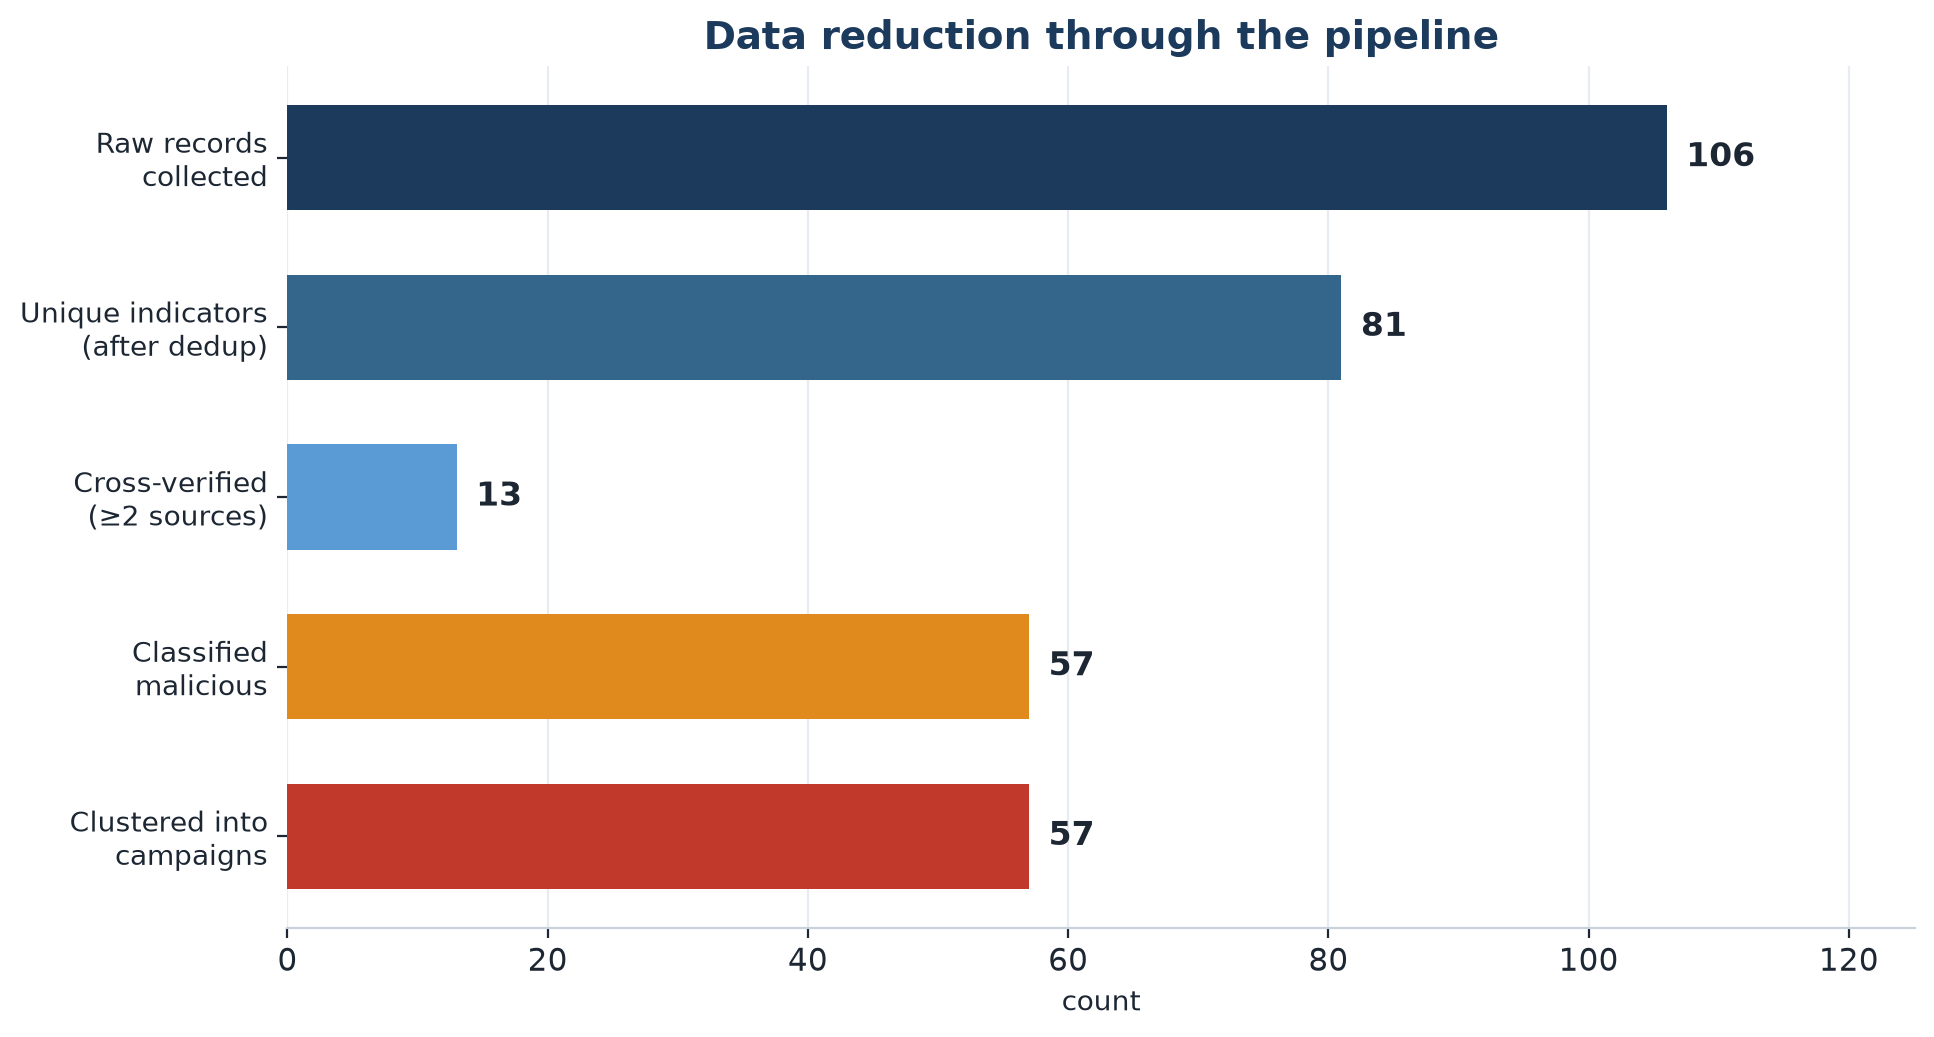
\includegraphics[width=0.92\linewidth]{figures/fig3_funnel.png}
\caption{Data reduction through the pipeline. Deduplication collapses 106 raw
records to 81 unique indicators; 57 classified malicious, of which 57 are
clustered into 8 campaigns (every malicious indicator found a campaign).}
\label{fig:funnel}
\end{figure}

\subsection{Composition}
Figure~\ref{fig:dist} shows the type and verdict mix. IPv4 addresses dominate
(39 of 81), followed by URLs (30); the verdict split is 57 malicious to 24
benign, with no indicators in the ambiguous band.

\begin{figure}[htbp]
\centering
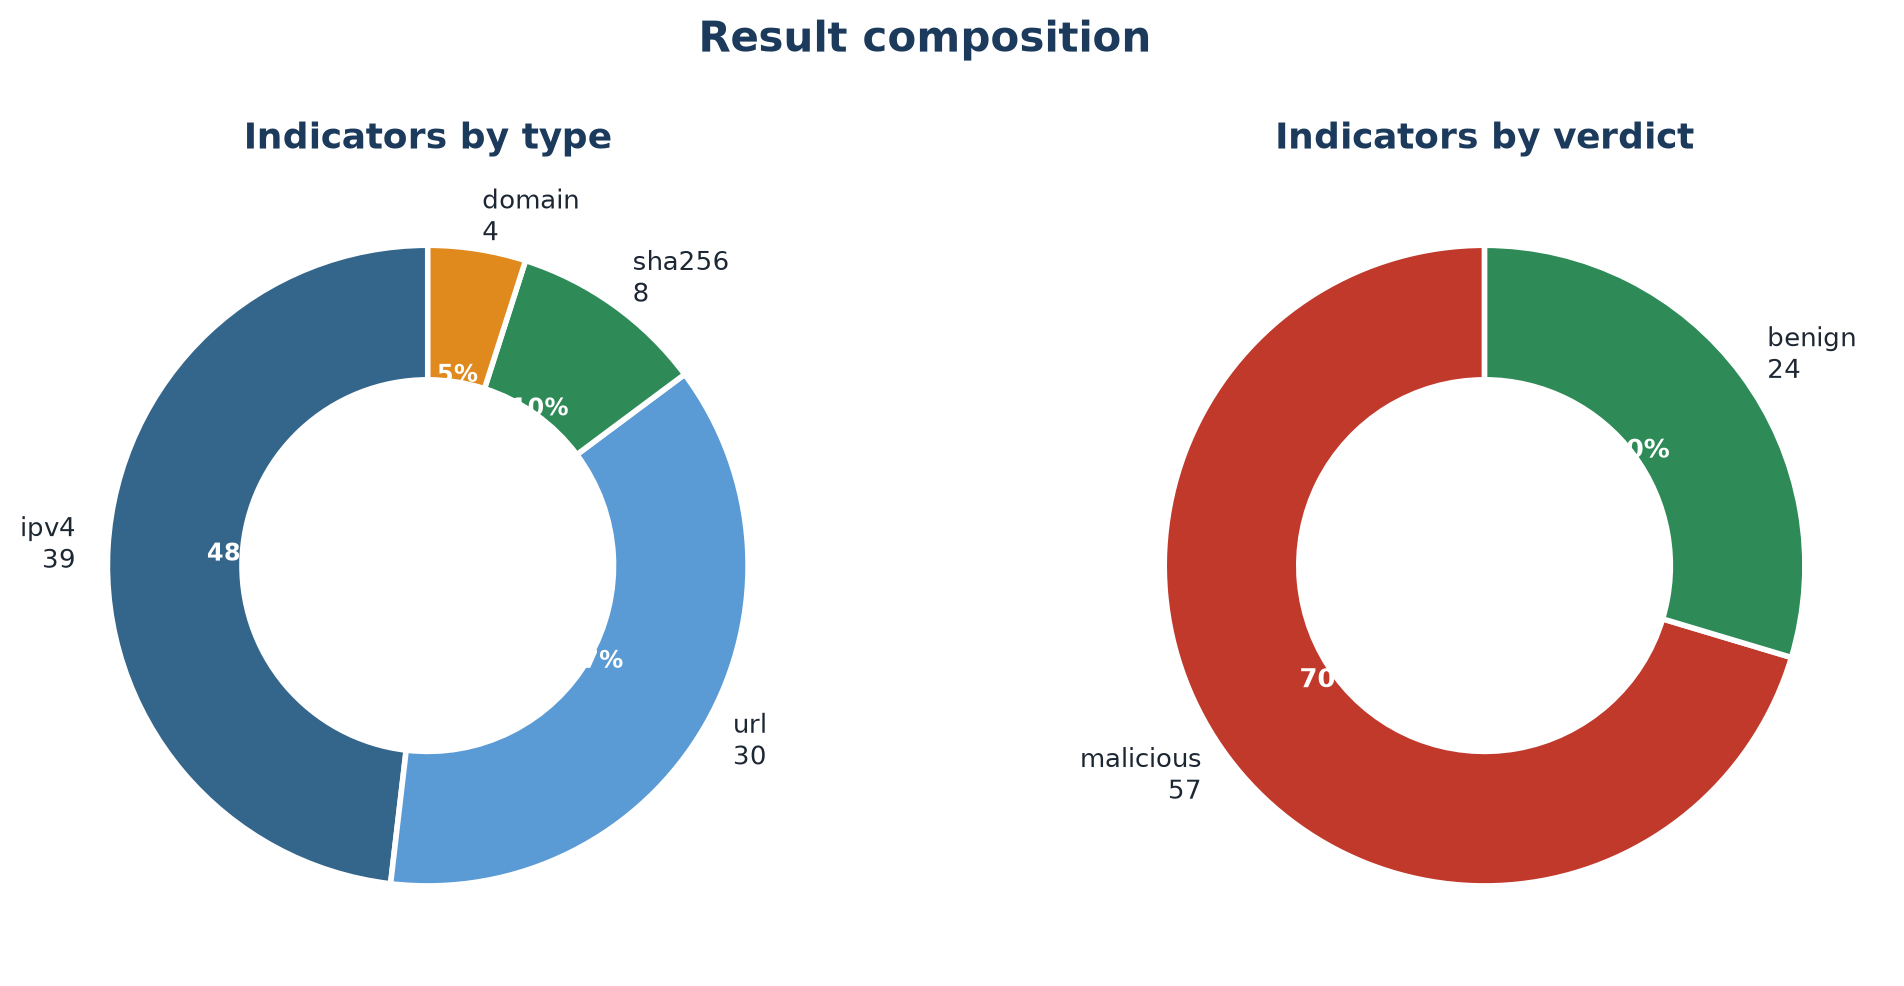
\includegraphics[width=\linewidth]{figures/fig4_distributions.png}
\caption{Indicator composition by type (left) and verdict (right).}
\label{fig:dist}
\end{figure}

\subsection{Source reliability}
The table and figure below show how each feed's static prior is adjusted by
measured behaviour. The internal honeypot has the lowest prior (0.70) but the
highest recall (1.00) and the best precision (0.565), so its dynamic evidence
pulls it well above its prior. Conversely Feodo keeps a high prior (0.90) and
ends with the top score (0.692) despite low precision --- the intended effect of
letting a strong prior resist a noisy batch.

\begin{figure}[htbp]
\centering
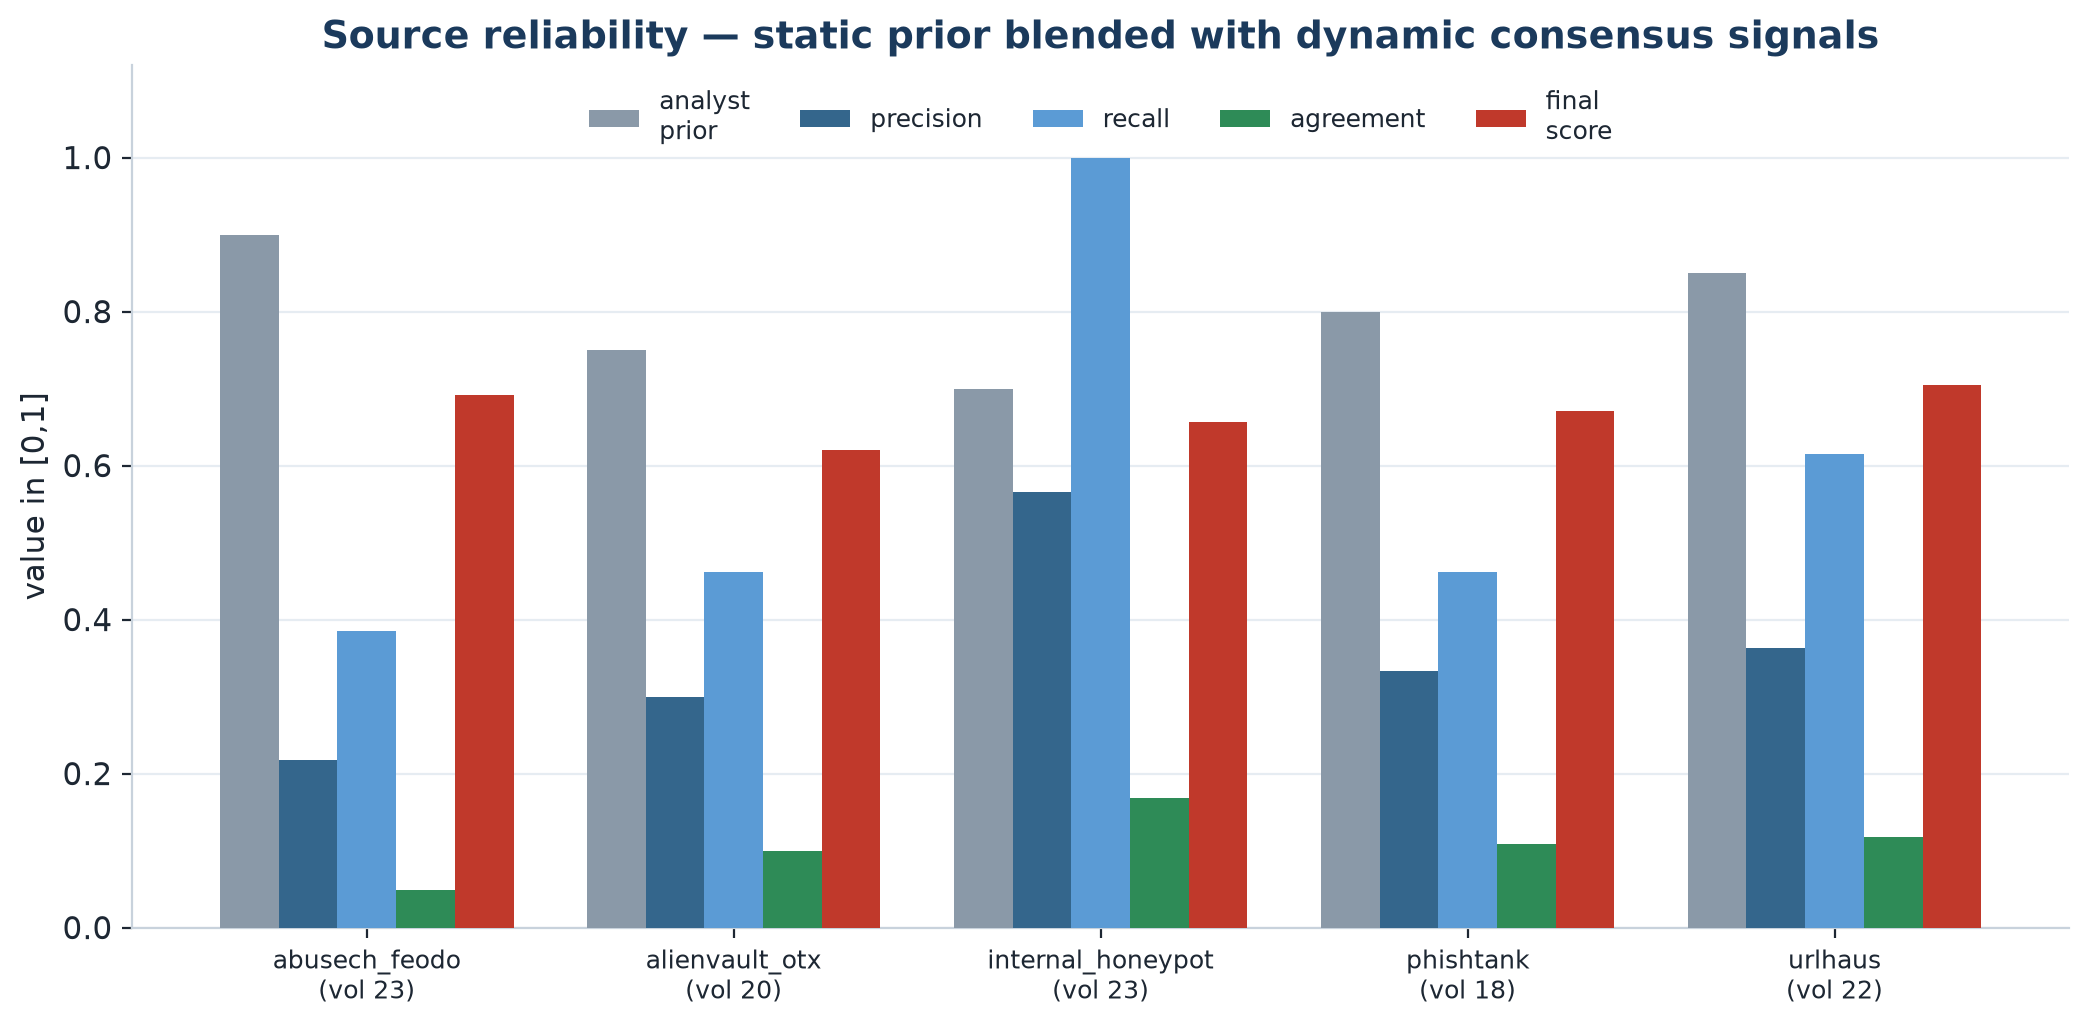
\includegraphics[width=\linewidth]{figures/fig5_source_reliability.png}
\caption{Source reliability. Prior, precision, recall, agreement and the blended
final score for each feed.}
\label{fig:rel}
\end{figure}

\begin{center}
\begin{tabular}{@{}lcccccc@{}}
\toprule
\rowcolor{paper}\textbf{Source} & \textbf{prior} & \textbf{prec.} & \textbf{recall} & \textbf{agree.} & \textbf{vol.} & \textbf{score} \\
\midrule
abusech\_feodo & 0.90 & 0.217 & 0.385 & 0.049 & 23 & \textbf{0.692} \\
urlhaus & 0.85 & 0.364 & 0.615 & 0.117 & 22 & \textbf{0.705} \\
phishtank & 0.80 & 0.333 & 0.462 & 0.108 & 18 & 0.671 \\
alienvault\_otx & 0.75 & 0.300 & 0.462 & 0.100 & 20 & 0.621 \\
internal\_honeypot & 0.70 & \textbf{0.565} & \textbf{1.000} & \textbf{0.168} & 23 & 0.656 \\
\bottomrule
\end{tabular}
\end{center}

\subsection{Classifier performance}
The classifier was evaluated on a held-out 25\% stratified test set. The
confusion matrix and ROC curve below were produced by replicating the exact
seeded split, so they match the reported metrics precisely.

\begin{figure}[htbp]
\centering
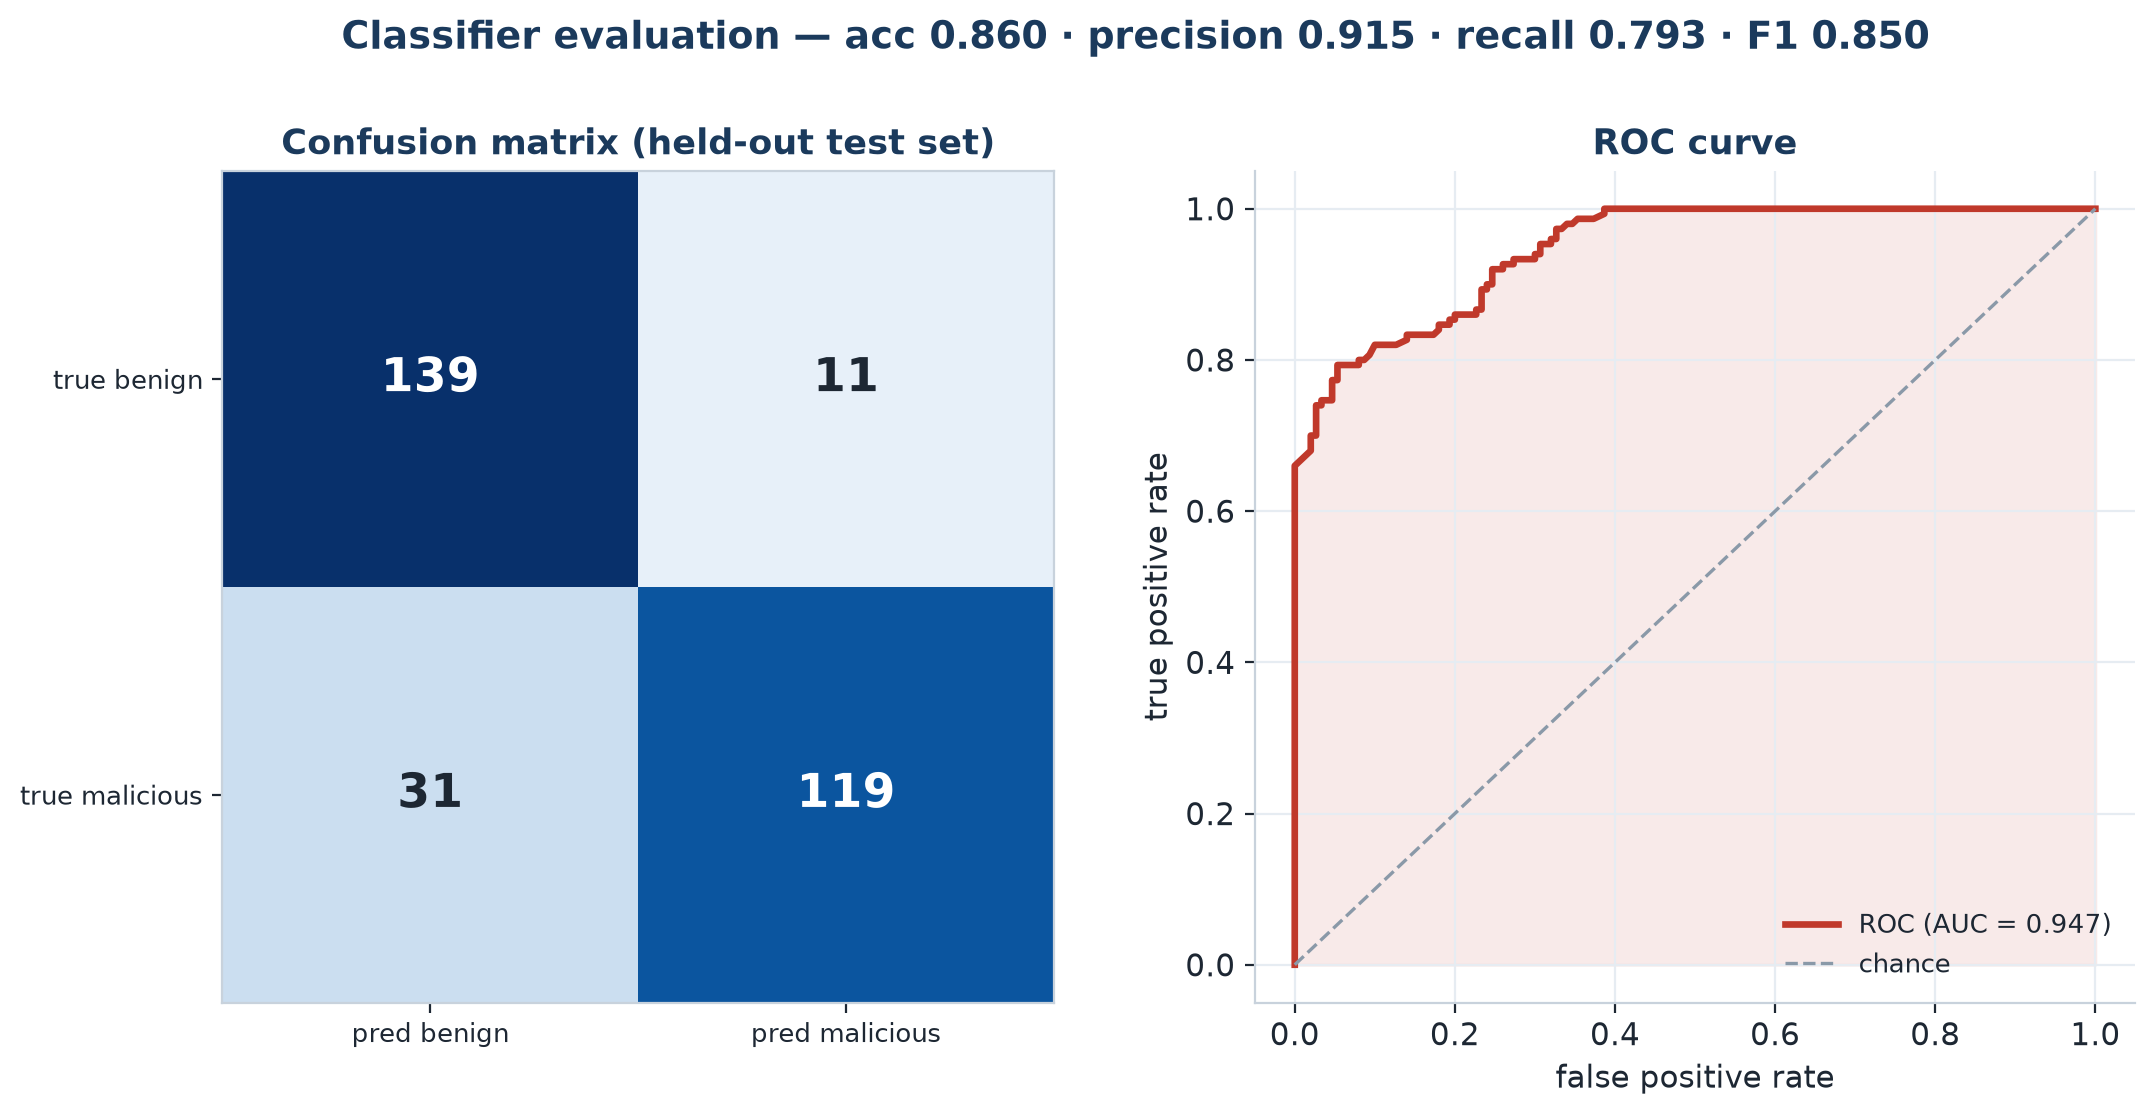
\includegraphics[width=\linewidth]{figures/fig7_classifier_eval.png}
\caption{Classifier evaluation. Left: confusion matrix on the held-out test set.
Right: ROC curve (AUC 0.946).}
\label{fig:eval}
\end{figure}

\begin{center}
\begin{tabular}{@{}lcccc@{}}
\toprule
\rowcolor{paper}\textbf{Metric} & \textbf{Accuracy} & \textbf{Precision} & \textbf{Recall} & \textbf{F1} \\
\midrule
Value & 0.860 & 0.915 & 0.793 & 0.850 \\
\bottomrule
\end{tabular}
\end{center}

The precision--recall asymmetry is deliberate and desirable for this domain:
precision (0.915) exceeds recall (0.793), meaning the model is conservative
about calling something malicious. In threat intelligence a false positive
(wasting analyst time, or worse, blocking a legitimate host) is costlier than a
miss, so this bias is the right one. ROC AUC of 0.946 indicates strong
separability overall.

\begin{figure}[htbp]
\centering
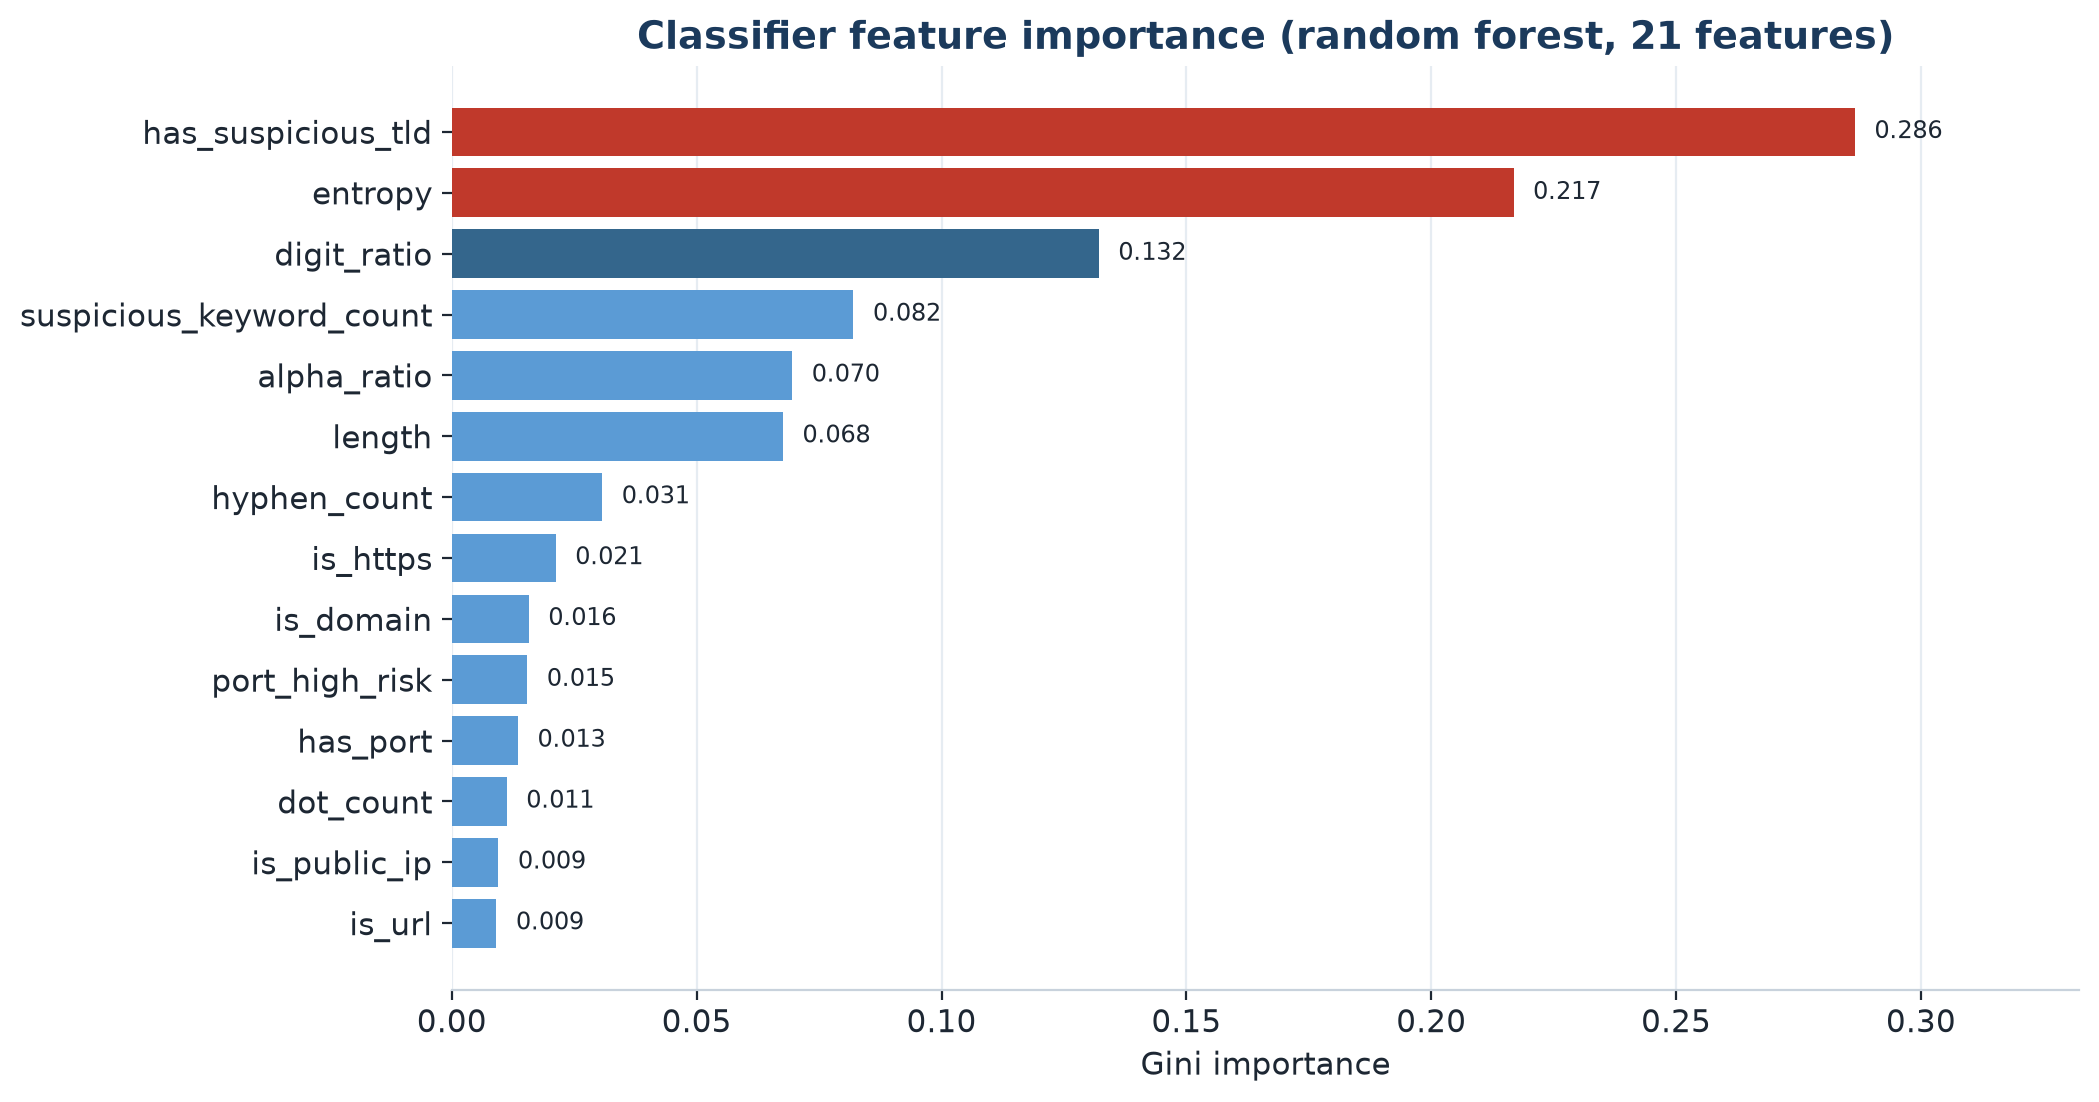
\includegraphics[width=0.94\linewidth]{figures/fig6_feature_importance.png}
\caption{Random-forest feature importance. The model relies most on
\code{has\_suspicious\_tld} (0.287), \code{entropy} (0.217) and
\code{digit\_ratio} (0.132) --- exactly the signals an analyst would use.}
\label{fig:imp}
\end{figure}

Feature importance (Figure~\ref{fig:imp}) confirms interpretability: the top
three signals are the suspicious-TLD flag, string entropy (DGA detection) and
digit ratio --- human-legible heuristics, not opaque interactions.

\subsection{Campaign clustering}
DBSCAN discovered 8 campaigns covering all 57 malicious indicators, with zero
noise points. The campaigns are coherent and map to recognisable threat
families.

\begin{figure}[htbp]
\centering
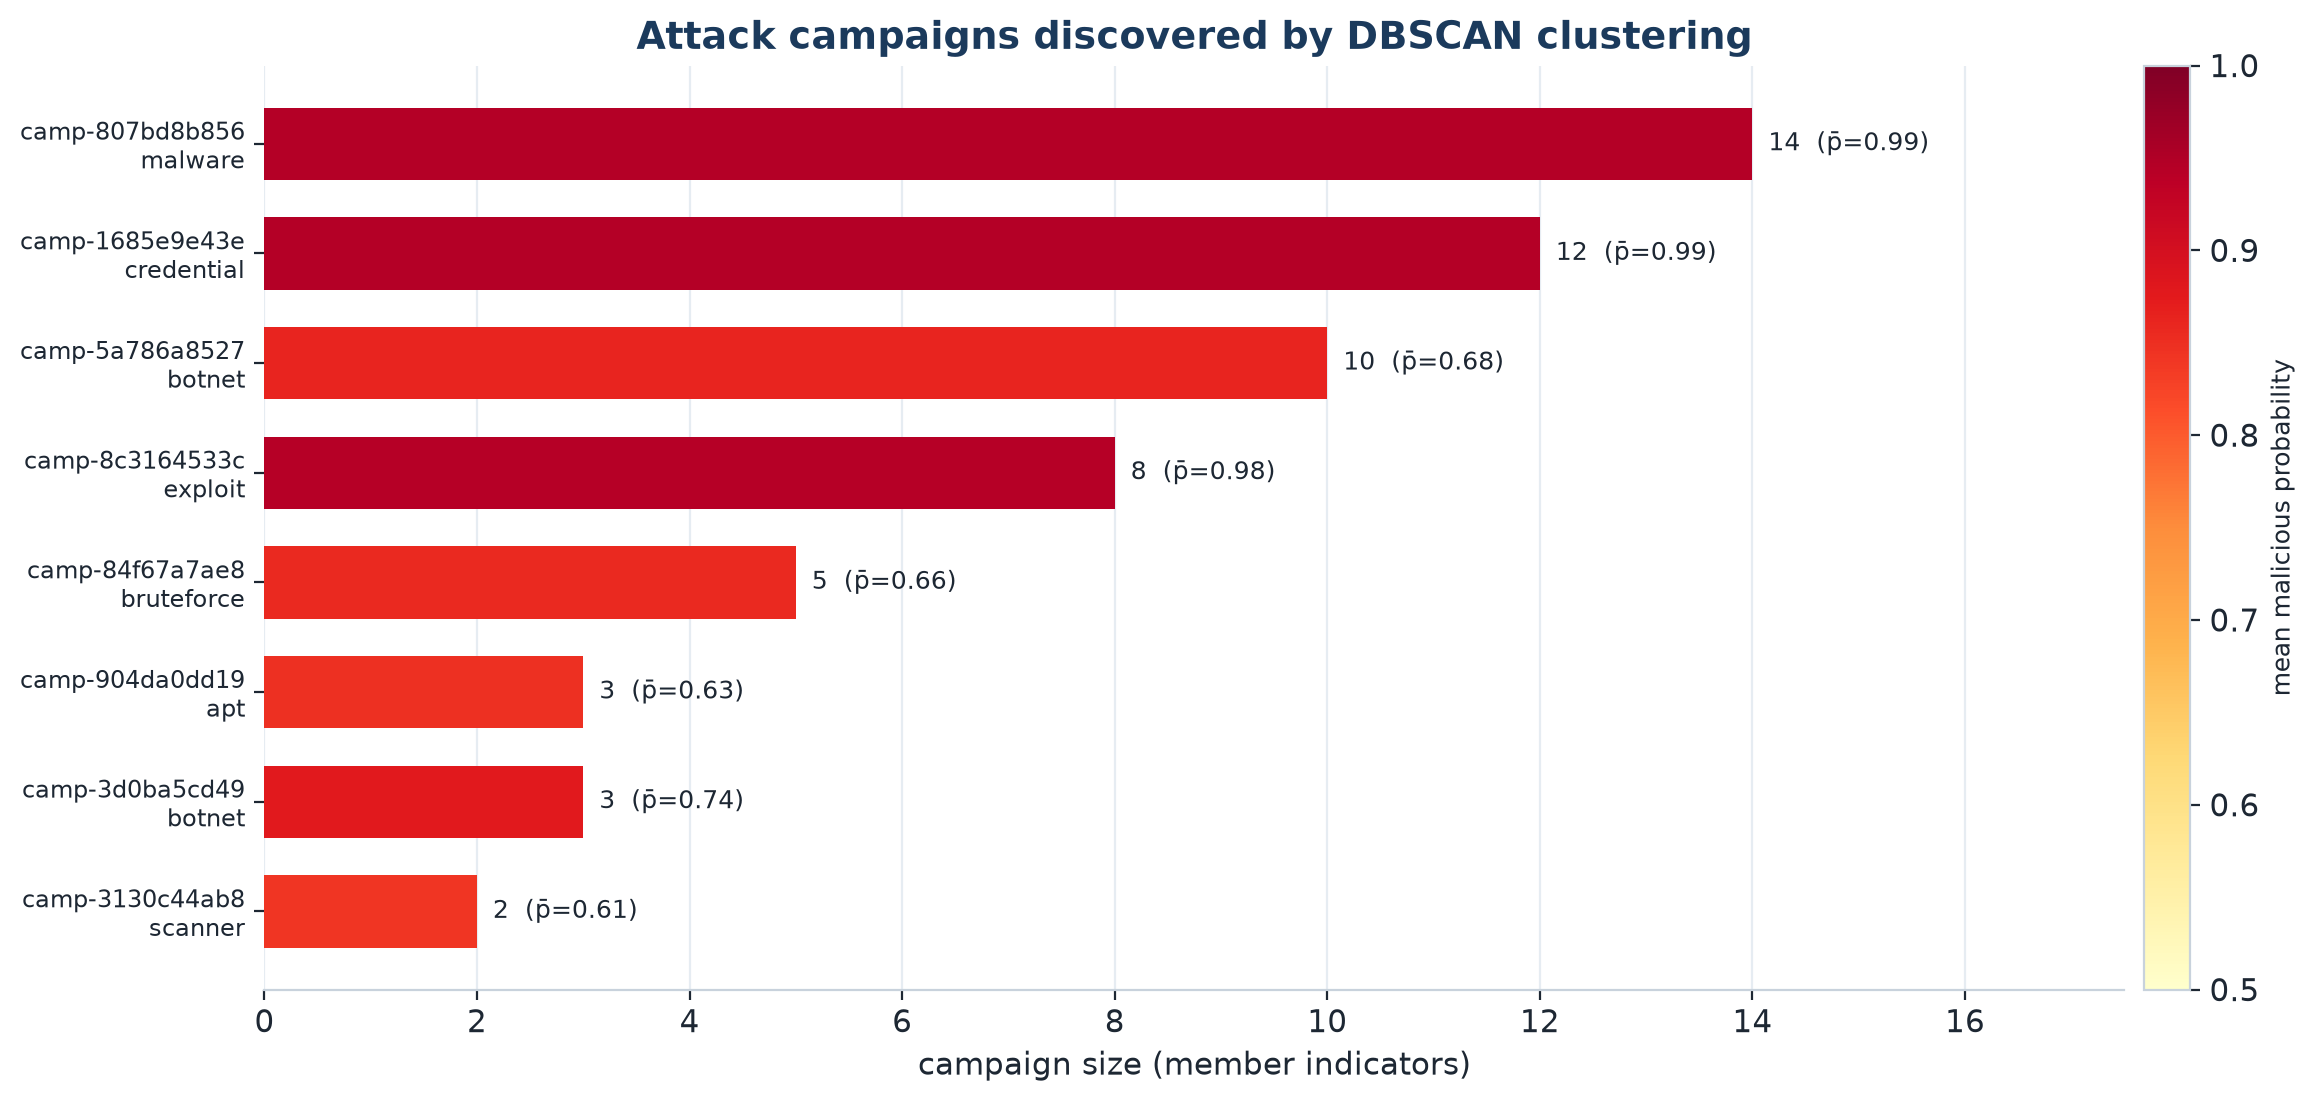
\includegraphics[width=\linewidth]{figures/fig8_campaigns.png}
\caption{Campaigns discovered by DBSCAN, sized by membership and coloured by mean
malicious probability. Labels derive from the most common shared tags.}
\label{fig:camp}
\end{figure}

\begin{center}
\begin{tabular}{@{}llcccl@{}}
\toprule
\rowcolor{paper}\textbf{Campaign} & \textbf{Label} & \textbf{Size} & \textbf{$\bar p$} & \textbf{$\bar r$} & \textbf{Shared tags} \\
\midrule
camp-807bd8b856 & malware & 14 & 0.99 & 0.82 & malware, payload \\
camp-1685e9e43e & credential & 12 & 0.99 & 0.84 & credential, phishing \\
camp-5a786a8527 & botnet & 10 & 0.68 & 0.90 & botnet, c2, trickbot \\
camp-8c3164533c & exploit & 8 & 0.98 & 0.88 & exploit, loader, payload, \dots \\
camp-84f67a7ae8 & bruteforce & 5 & 0.66 & 0.60 & bruteforce, honeypot \\
camp-3d0ba5cd49 & botnet & 3 & 0.74 & 0.90 & botnet, c2, emotet, apt \\
camp-904da0dd19 & apt & 3 & 0.63 & 0.70 & apt, malware \\
camp-3130c44ab8 & scanner & 2 & 0.61 & 0.60 & scanner \\
\bottomrule
\end{tabular}
\end{center}

\begin{keybox}[Campaign IDs are reproducible]
Because a campaign's ID is a hash of its members' stable indicator IDs, the same
input data always produces the same campaign identifiers. This makes it possible
to track a campaign's evolution across runs --- an important property for
operational use that a naive random cluster label would not provide.
\end{keybox}

\subsection{Per-feed contribution}
Finally, Figure~\ref{fig:contrib} shows how much each feed contributes and how
much survives deduplication --- the practical measure of feed overlap.

\begin{figure}[htbp]
\centering
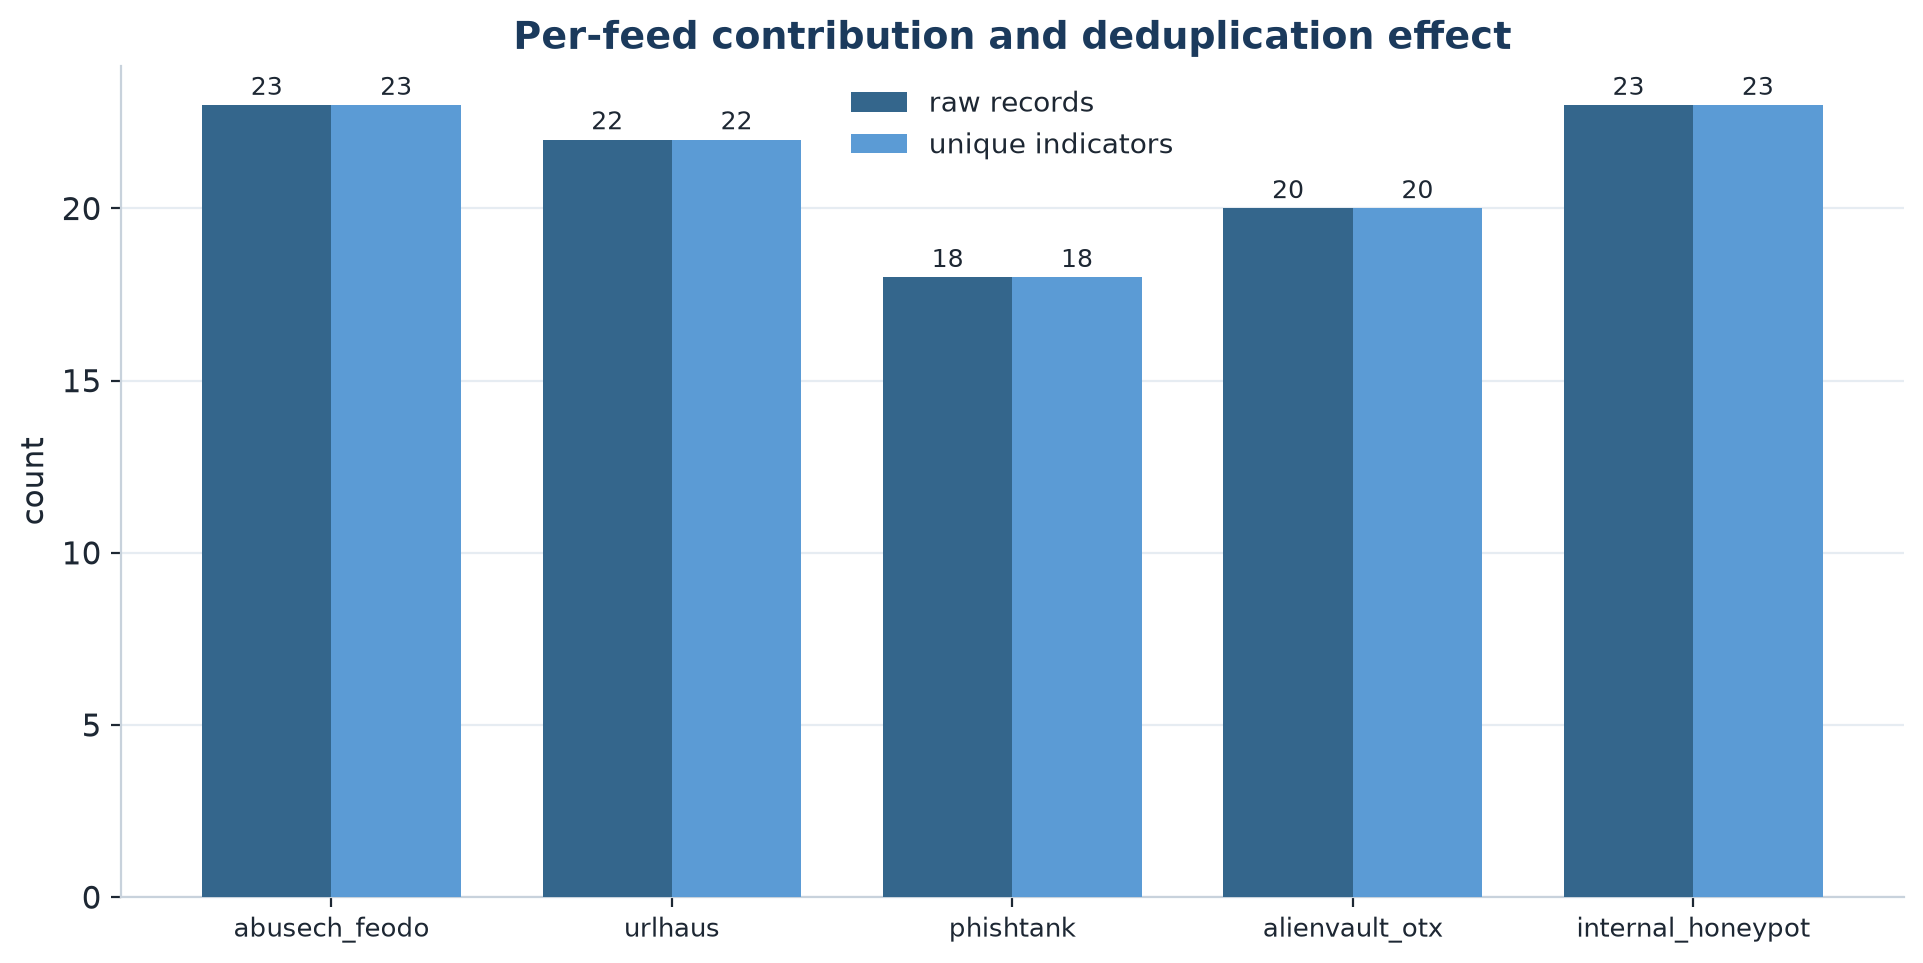
\includegraphics[width=0.95\linewidth]{figures/fig9_contribution.png}
\caption{Raw records versus unique indicators contributed per feed. The gap is
the overlap that manual triage would otherwise reconcile by hand.}
\label{fig:contrib}
\end{figure}

% ============================== 9. INTERFACES ==============================
\section{Interfaces, Deployment and Reproducibility}

\subsection{Command-line interface}
\begin{lstlisting}[language=bash]
# Deterministic offline run (the reference run in this report)
threatint --offline

# Live feeds, with per-source fixture fallback on any failure
threatint

# Train on analyst-reviewed labels and persist the model
threatint --labels labels.csv --model-path artifacts/classifier.joblib

# Reuse a saved model without retraining; export machine-readable output
threatint --use-saved-model --out-json out.json --out-indicators iocs.csv
\end{lstlisting}

\subsection{Web dashboard and static export}
\begin{lstlisting}[language=bash]
threatint-web --offline --port 12000        # live Flask console + JSON API
threatint-static --offline --out dist/index.html   # single-file HTML export
\end{lstlisting}

The dashboard is a read-only ``operations console'': an indicators table with
probability, verdict, type, source count, reliability and campaign, filterable
and paginated; a campaign grid; and a source-reliability ranking. All indicator
values are defanged before display.

\subsection{Deployment paths}
Three deployment paths ship in the repository, all exercised during development:

\begin{center}
\begin{tabularx}{\linewidth}{@{}>{\bfseries}p{3.4cm}X@{}}
\toprule
\rowcolor{paper}\textbf{Path} & \textbf{Mechanism} \\
\midrule
GitHub Pages & \code{publish-dashboard.yml} renders the static console and publishes it on push to \code{main}. No server, no secrets. \\
Docker & \code{Dockerfile} installs the package, bakes a static dashboard into the image, and serves the live console on port 12000. \\
CI & \code{ci.yml} runs \code{pyflakes} and the full \code{pytest} suite on Python 3.10 and 3.12. \\
\bottomrule
\end{tabularx}
\end{center}

\subsection{Testing}
The suite comprises \textbf{60 tests} across eight modules (models, normalize,
features, classifier, clustering, verification, pipeline, webapp), all running
offline and deterministically. Lint is clean under \code{pyflakes}. The tests
assert real behaviour, not mocks: the end-to-end test runs the whole pipeline
and checks that a deliberately shared indicator is reported by at least three
sources.

% ============================== 10. SECURITY ===============================
\section{Security Considerations}

Because the system handles indicators that are themselves adversarial strings,
several precautions matter:

\begin{itemize}[leftmargin=1.4em,itemsep=3pt]
  \item \textbf{Defanging on display.} The dashboard renders every indicator
    defanged (\code{hxxp://\dots[.]}) so a live IOC is never a clickable link.
  \item \textbf{Output escaping.} Indicator text is escaped client-side before
    insertion into the DOM, preventing stored-XSS via a malicious feed.
  \item \textbf{No remote reconfiguration.} The web layer accepts only
    pagination and filter parameters; the pipeline cannot be steered remotely.
  \item \textbf{Least-privilege API keys.} Live feed credentials are read from
    environment variables named in config, never hard-coded.
  \item \textbf{Bounded inputs.} API page size is clamped ($\le 500$); offset is
    non-negative; malformed integers fall back to safe defaults.
  \item \textbf{Provenance retained.} Raw payloads are preserved, so every
    downstream decision can be audited back to its source record.
\end{itemize}

% ============================== 11. LIMITATIONS ============================
\section{Limitations}

Honest scoping matters more than a flattering one. The principal limitations:

\begin{enumerate}[leftmargin=1.4em,itemsep=3pt]
  \item \textbf{The default model trains on synthetic data.} The reported
    metrics characterise the pipeline, not production accuracy. Real use
    requires analyst-reviewed labels via \code{--labels}; the interface is ready
    and the report always records \code{data\_source}.
  \item \textbf{The reference run is small and offline.} 81 indicators is enough
    to exercise every stage, not to characterise feed-scale behaviour. A live
    validation did ingest 32{,}289 URLhaus records and 106{,}407 records in
    total, demonstrating scale, but that run is not the basis of these metrics.
  \item \textbf{Agreement is corpus-relative.} Precision/recall are measured
    against a consensus that itself assumes majority-correctness; a
    systematically wrong majority would propagate.
  \item \textbf{No temporal decay.} Features include indicator age, but source
    reliability is not yet time-weighted; a feed that was good last year scores
    the same as one that is good today.
  \item \textbf{Clustering distance is heuristic.} The lexical/tag blend and its
    0.6/0.4 weighting are principled but not learned or tuned against labelled
    campaigns.
\end{enumerate}

% ============================== 12. FUTURE WORK ============================
\section{Future Work}

\begin{itemize}[leftmargin=1.4em,itemsep=3pt]
  \item \textbf{Analyst-labelled training loop}: feed confirmed/denied verdicts
    back as labels, with periodic retraining and drift monitoring.
  \item \textbf{Temporal source weighting}: exponentially decay historical
    agreement so reliability tracks a feed's current behaviour.
  \item \textbf{Graph-based campaign linking}: model shared infrastructure
    (registrar, ASN, certificate, hosting) as a graph to link campaigns beyond
    lexical/tag similarity.
  \item \textbf{Enrichment}: passive-DNS, WHOIS and certificate-transparency
    lookups to strengthen weak signals for low-reliability indicators.
  \item \textbf{Explainability surface}: expose per-indicator feature
    contributions (e.g.\ SHAP) directly in the dashboard so an analyst sees
    \emph{why} the model scored something.
  \item \textbf{Feed-scale evaluation}: rerun the full metrics against a large,
    labelled, live corpus and publish calibration curves.
\end{itemize}

% ============================== 13. CONCLUSION =============================
\section{Conclusion}

ThreatInt demonstrates that the mechanical layer of threat triage ---
collection, reconciliation, scoring and grouping --- can be automated into a
small, reproducible, well-tested system. Its distinguishing qualities are not
exotic algorithms but sound engineering: computed (not assumed) trust,
network-optional determinism, interpretable features, and honest labelling of
synthetic data. On the reference run it turns 106 records from five disagreeing
feeds into 81 deduplicated indicators, 57 classified malicious with 0.946 AUC,
and 8 coherent attack campaigns with reproducible identifiers --- while running
offline, in CI, and on a laptop.

The system is deliberately a foundation. The path to production is clear and
mostly about data, not architecture: point \code{--labels} at analyst-reviewed
ground truth, widen the corpus, and add temporal and graph-based enrichment.
The pipeline is built so those upgrades drop in without redesign.

% ============================== APPENDICES =================================
\appendix
\section{Configuration Reference}
\begin{lstlisting}[language=Python]
pipeline:
  min_sources_for_verification: 2      # consensus threshold m
  malicious_threshold: 0.5             # verdict cutoff theta
  min_reliability_for_clustering: 0.35 # clustering eligibility floor
  random_seed: 42                      # determinism

sources:                               # name / kind / prior / url / fixture
  - abusech_feodo   (domain, 0.90)     # feodotracker blocklist
  - urlhaus         (url,    0.85)     # urlhaus recent URLs
  - phishtank       (url,    0.80)     # phishtank online-valid
  - alienvault_otx  (mixed,  0.75)     # OTX pulses
  - internal_honeypot (mixed, 0.70)    # local captures (no URL)

features:   suspicious_tlds, suspicious_keywords, high_risk_ports
ml:         model, n_estimators, max_depth, test_size, model_path
clustering: eps: 0.22, min_samples: 2   # DBSCAN parameters
\end{lstlisting}

\section{CLI Reference}
\begin{center}
\begin{tabularx}{\linewidth}{@{}>{\ttfamily\small}p{4.3cm}X@{}}
\toprule
\rowcolor{paper}\textbf{Flag} & \textbf{Purpose} \\
\midrule
--config PATH & Config file (defaults to repo config). \\
--offline & Use bundled fixtures only; never touch the network. \\
--labels PATH & Analyst labels CSV (indicator, label) for supervised training. \\
--model-path PATH & Where to save/load the trained classifier. \\
--use-saved-model & Load a saved model instead of retraining. \\
--no-train & Skip training (verdicts stay UNKNOWN). \\
--corpus-size N & Synthetic bootstrap corpus size (default 1200). \\
--out-json / --out-indicators / --out-campaigns & Machine-readable exports. \\
--top N & Rows in the console report. \\
--quiet / -v & Minimal output / debug logging. \\
\bottomrule
\end{tabularx}
\end{center}

\section{Reproducing This Report}
\begin{lstlisting}[language=bash]
python -m venv .venv && .venv/bin/pip install -e ".[dev,web]"
.venv/bin/python -m pytest -q                 # 60 tests
.venv/bin/threatint --offline                 # the reference run
.venv/bin/python report/make_figures.py       # regenerate every figure
.venv/bin/python report/build_report.py       # compile this PDF
\end{lstlisting}

\vspace{0.6cm}
\begin{center}
\rule{8cm}{0.4pt}\\[0.25cm]
{\footnotesize\color{grey}
ThreatInt v0.1.0 · Technical Research Report · all metrics from a deterministic
offline run (seed 42)}
\end{center}

\end{document}
